\documentclass[9pt,twocolumn,twoside]{pnas-new}
% Use the lineno option to display guide line numbers if required.
% Note that the use of elements such as single-column equations
% may affect the guide line number alignment.

\templatetype{pnasresearcharticle} % Choose template
% {pnasresearcharticle} = Template for a two-column research article
% {pnasmathematics} = Template for a one-column mathematics article
% {pnasinvited} = Template for a PNAS invited submission

\usepackage{pslatex}
\usepackage{amsfonts}
\usepackage{graphicx}
\usepackage{color}
\usepackage{todonotes}
\usepackage{dsfont}
\usepackage{array}
\usepackage{textcomp}
\usepackage{multirow}
\usepackage{subfig}
\usepackage{todonotes}
\usepackage{hyperref}

\newcommand{\mwu}[1]{{\color{green}{[mwu: #1]}}}

\title{Contextual flexibility in visual communication}

% Use letters for affiliations, numbers to show equal authorship (if applicable) and to indicate the corresponding author

\author[a,1]{Judith E. Fan}
\author[a]{Robert X.D. Hawkins}
\author[b]{Mike Wu}
\author[a,b]{Noah D. Goodman}

\affil[a]{Department of Psychology, Stanford University}
\affil[b]{Department of Computer Science, Stanford University}

% Please give the surname of the lead author for the running footer
\leadauthor{Fan}

\significancestatement{Drawing is a versatile tool for communication, spanning detailed life drawings and simple whiteboard sketches. Even the same object can be drawn in many ways, depending on the context. How do people decide how to draw in order to be understood? We collected a large number of drawings in different contexts and found that people adapted their drawings accordingly, producing detailed drawings when necessary, but simpler drawings when sufficient. To explain this contextual flexibility, we developed a computational model combining the capacity to perceive the correspondence between an object and drawing with the ability to infer what information is relevant to the viewer in context. Our results suggest drawing may be so versatile because of humans' joint capacity for visual abstraction and social inference.}

% Please include corresponding author, author contribution and author declaration information
\authorcontributions{J.E.F and R.X.D.H. conducted human experiments, J.E.F, R.X.D.H, and M.W. analyzed data and performed computational modeling. J.E.F, R.X.D.H, M.W., and N.D.G. designed experiments, formulated models, interpreted results, and wrote the paper.}
\authordeclaration{The authors declare no conflict of interest.}
\correspondingauthor{\textsuperscript{1}To whom correspondence should be addressed. E-mail: jefan@stanford\@email.edu}

% Keywords are not mandatory, but authors are strongly encouraged to provide them. If provided, please include two to five keywords, separated by the pipe symbol, e.g:
\keywords{drawing $|$ deep learning $|$ pragmatics $|$ computational modeling $|$ Rational Speech Act frameowrk}

\begin{abstract}
Visual modes of communication are ubiquitous in modern life --- from maps to data plots to political cartoons. 
Here we investigate drawing, the most basic form of visual communication. 
Communicative drawing poses a core challenge for theories of how vision and social cognition interact, requiring a detailed understanding of how sensory information and social context jointly determine what information is relevant to communicate. 
Participants (N=192) were paired in an online environment to play a drawing-based reference game. On each trial, both participants were shown the same four objects, but in different locations. The \textit{sketcher's} goal was to draw one of these objects --- the target --- so that the \textit{viewer} could pick it out from a set of distractor objects. 
There were two types of trials: close, where objects belonged to the same basic-level category (i.e., bird, car, chair, dog), and far, where objects belonged to different categories. 
We found that people exploited information in common ground with their partner to efficiently communicate about the target: on far trials, sketchers achieved 99.7\% recognition accuracy while applying fewer strokes, using less ink, and spending less time (\textit{p}s$<$0.001) on their drawings than on close trials. 
We hypothesized that humans excel at this task by recruiting two core competencies: (1) \textbf{visual abstraction}, the capacity to perceive the correspondence between an object and a drawing of it; and (2) \textbf{pragmatic inference}, the ability to infer what information would help a viewer distinguish the target from distractors. 
We instantiated these competencies in a computational model that combines a deep convolutional neural network visual encoder with a Bayesian model of recursive social reasoning, and found that it fit the data well and outperformed lesioned variants of the model. 
Together, this work provides the first unified computational theory of how perception and social cognition support contextual flexibility in real-time visual communication.
\end{abstract}

\dates{This manuscript was compiled on \today}
\doi{\url{www.pnas.org/cgi/doi/10.1073/pnas.XXXXXXXXXX}}

\begin{document}

% Optional adjustment to line up main text (after abstract) of first page with line numbers, when using both lineno and twocolumn options.
% You should only change this length when you've finalised the article contents.
\verticaladjustment{-2pt}

\maketitle
\thispagestyle{firststyle}
\ifthenelse{\boolean{shortarticle}}{\ifthenelse{\boolean{singlecolumn}}{\abscontentformatted}{\abscontent}}{}

%%%%% In another version of the intro, you recap the visual production stuff on its own, and then point out that drawing is not one task, but several, and could depend a lot of the goals and context, and in this paper, we extend previous models to handle this.

A watershed moment in the history of human cognition and culture was the invention of graphical representation, independently in Europe and Asia, about 30-60 thousand years ago \cite{hoffmann2018u,Aubert:2014jy}. 
Graphical representation was transformative because it provided a means for people to encode their thoughts in a durable and shareable format \cite{donald1991origins}. 
From ancient etchings on cave walls to modern digital displays, using graphical representations for visual communication lies at the heart of key human innovations (e.g., mapmaking, data visualization), and forms the foundation for the cultural transmission of knowledge and higher-level reasoning \cite{tomasello2009cultural,card1999readings}. 
Drawing, in which a person produces marks that form a meaningful image, is a particularly important case study for understanding human visual communication. Drawn images predate symbolic writing systems \cite{clottes2008cave}, are pervasive in many cultures \cite{gombrich1989story}, and are produced prolifically by children from an early age \cite{kellogg1969analyzing}.

Remarkably, we perceive drawings of objects as resembling physical objects in spite of the fact that drawings and objects are profoundly different in composition. 
What explains their effectiveness for conveying visual concepts? 
One hypothesis explored in prior work is that the ability to perceive the correspondence between drawings and real-world objects arises from a common, general-purpose neural architecture evolved to handle natural visual inputs \cite{Sayim:2011bz,gibson2014ecological}. 
In support of this hypothesis, it was recently shown that features learned by deep convolutional neural network models (DCNNs) trained exclusively to recognize objects in photos and had never seen a line drawing succeed in recognizing simple sketches \cite{FanCommon2018,yamins2014performance}. 
These results are consistent with evidence from other domains, including developmental, cross-cultural, and comparative studies of drawing perception. 
For example, human infants \cite{hochberg1962pictorial}, people living in remote regions without pictorial art traditions and without substantial contact with Western visual media \cite{kennedy1975outline}, and higher non-human primates \cite{tanaka2007recognition} are able to recognize line drawings of familiar objects, even without prior experience with drawings. 
Together, these findings suggest that a thorough understanding of the functional architecture of the visual system, which is largely shared across human cultures, may be sufficient to explain how people are able to perceive semantic content in drawings.

However, such an explanation is clearly incomplete. 
Even drawings of the same object can be highly variable \cite{quickdraw2017}, illustrating the importance of other factors that may influence how a drawing conveys meaning. 
For example, extended visual communication within a community may lead to the formation of culturally-specific graphical conventions over the course of several generations \cite{toku2001cross,boltz1994origin}. 
Recent laboratory studies of visual communication have also provided experimental evidence that pairs of interacting participants can, over the course of minutes, learn to produce drawings that are referentially meaningful to their partner in context, even when these drawings do not strongly resemble any particular real-world referent out of context \cite{Garrod:2007wk,fay2010interactive,Galantucci:2005uh,Healey:2007vq}. 
Together, findings in this literature suggest the importance of social context --- and over longer timescales, culturally shared conventions --- in determining how drawings convey meaning.

Building on this prior work, the current study is guided by the overarching hypothesis that successful visual communication by drawing recruits pragmatic reasoning \cite{goodman2016pragmatic,clark1996using,wilson1986relevance,grice1975syntax} --- the ability to determine which information is not only \textit{valid} to include in a drawing, but also \textit{relevant} in context --- in combination with visual perception --- the set of computations that transform raw visual inputs into semantically meaningful internal representations.

To investigate visual communication in a naturalistic yet controlled setting, here we employ sketching-based reference games. 
These reference games involve two players: a sketcher who aims to help a viewer pick out a target object from an array of alternative, distractor objects by representing it in a sketch. 
This basic arrangement can be traced back to the language games explored by \citep{wittgenstein1953philosophical} and \citep{Lewis69_Convention}. 
Such games have proven to be a valuable tool for eliciting pragmatic inferences about \textit{language} use in context, and to make quantitative measurements of the behavioral consequences of these inferences \cite{goodman2016pragmatic,kao2014formalizing,goodman2013knowledge,frank2012predicting}. 
Here we generalize this methodology to understand how sketchers account for information in common ground with their viewer in order to produce sketches that are informative \cite{grice1975syntax,wilson1986relevance} yet parsimonious \cite{zipf1936psycho}.

Traditionally, a barrier to progress in studying visual communication has been the lack of principled quantitative measures of high-level semantic information in drawings. 
As such, previous studies employing drawing tasks to study visual communication have typically relied on qualitative assessments of drawings based on provisional criteria specific to each study \cite{Healey:2007vq}, or quantitative measures of low-level visual features that do not capture semantic information \cite{Garrod:2007wk}, limiting their ability to make detailed, quantitative predictions about visual communication behavior.

The goal of this paper is to provide a computational framework for systematically investigating how social context influences how people convey visual concepts in real-time. 
We present an integrated computational model of contextual flexibility in visual communication that combines deep convolutional neural network models of visual perception with a Bayesian probabilistic model of pragmatic reasoning \cite{goodman2016pragmatic} to make detailed quantitative predictions of what drawings people will produce across a variety of communicative contexts. 
We found that our full model fits the data well and outperformed lesioned variants.

\section*{Results}

\subsection*{Effect of context manipulation on communication task performance}

%%%%% List of results figures
%% Figure 1: Task Display & Design & example drawings
%% Figure 2: Sketch Gallery
%% Figure 3: Communication Game Task Performance & Recognition Task Performance
%% Figure 4: Model schematic
%% Figure 5: Model comparison & evaluation (absolute performance) -- human+RSA (2 production x 2 pragmatics = 4 bars) + VGG+RSA (2 production x 2 pragmatics x 3 perception = 12 bars)

%% Supplemental 1: Perceptual similarity -- maybe confusion matrix
%% Supplemental 2: Param posteriors
%% Supplemental 3: Error analysis for each lesioned versions

\begin{figure*}[htbp]
\centering
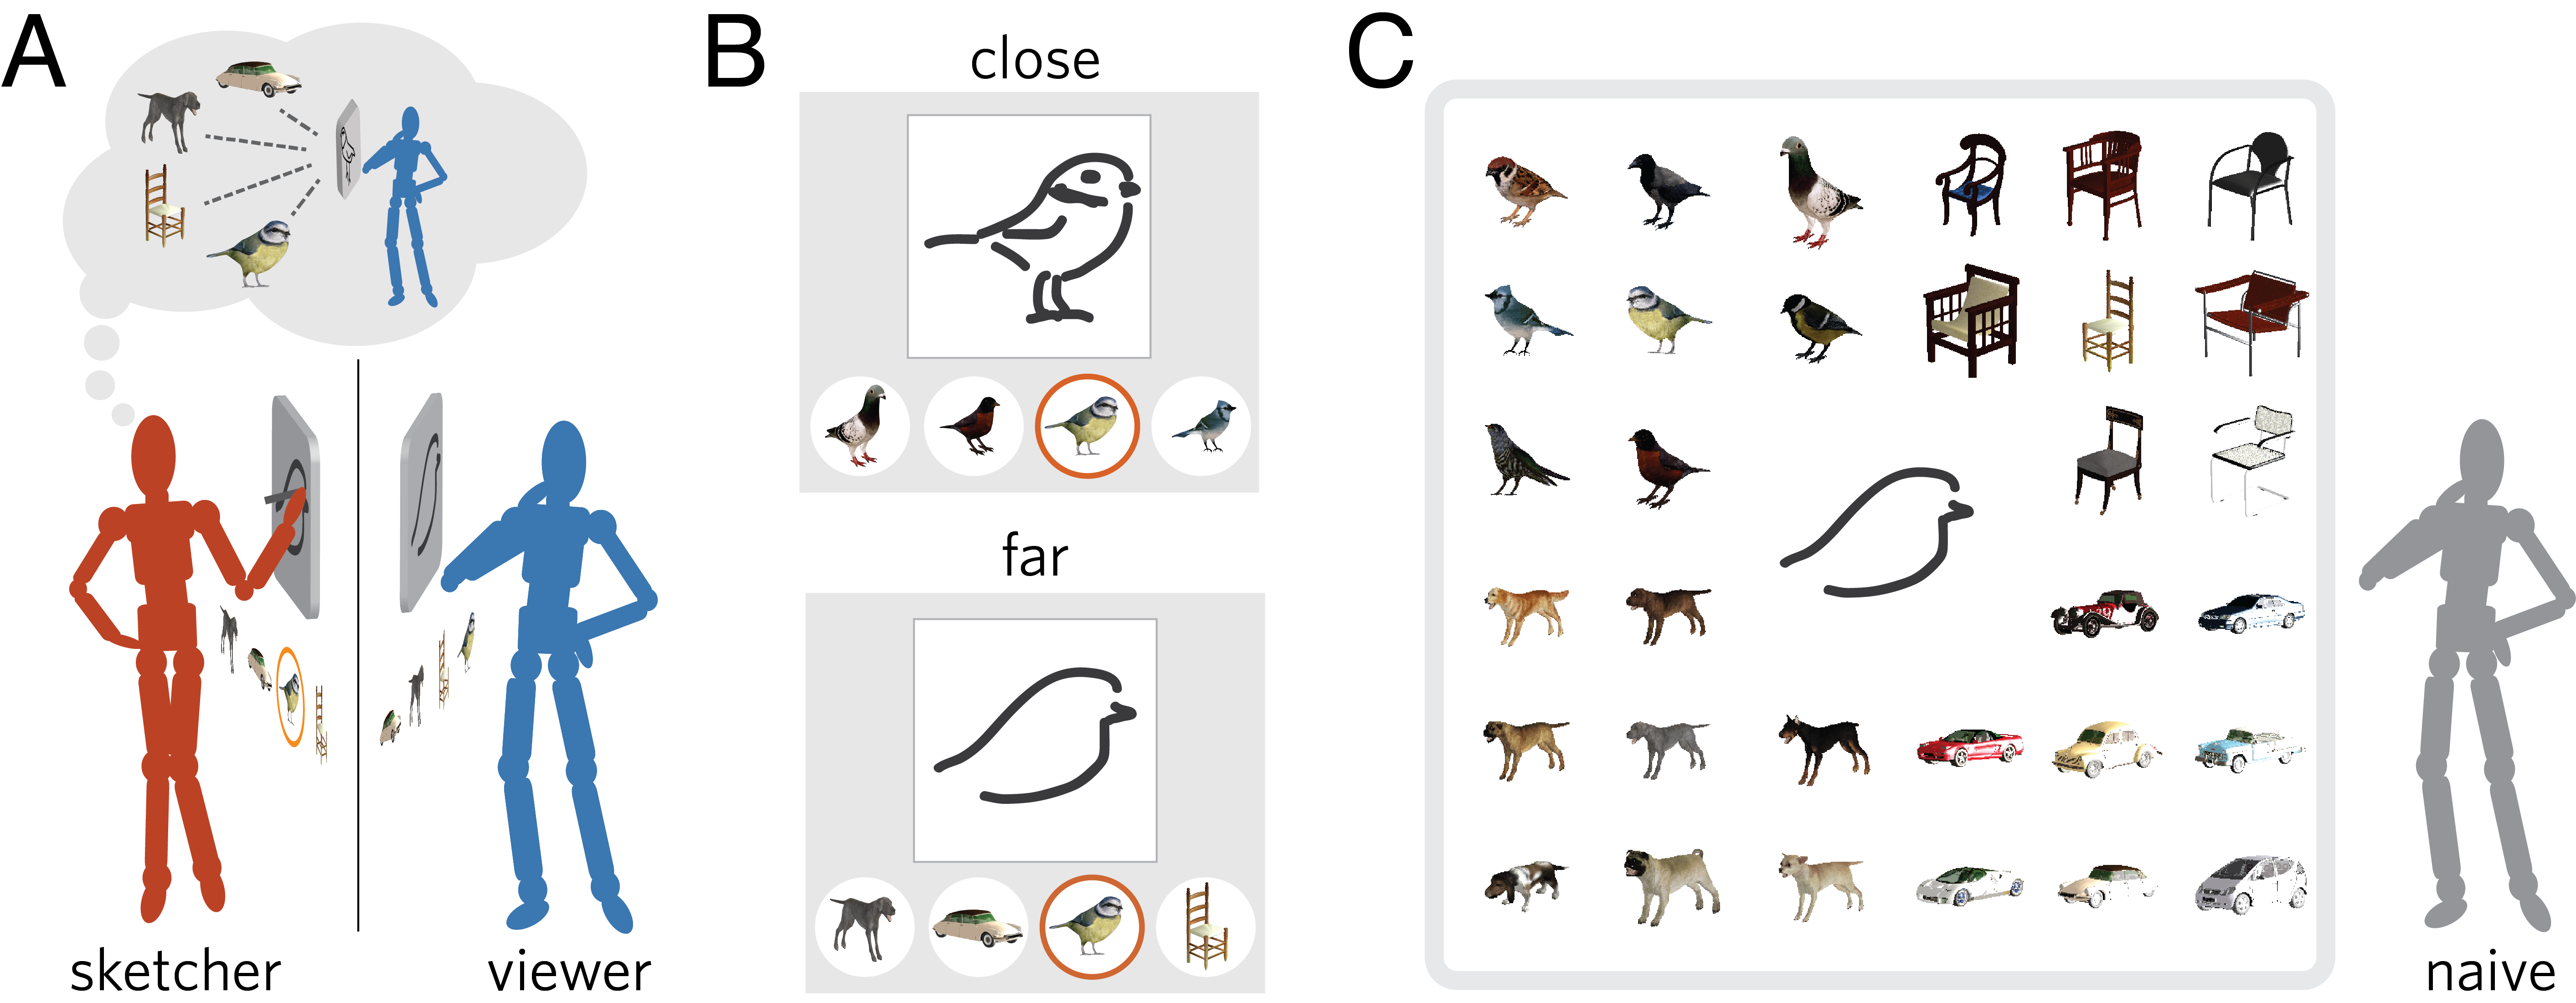
\includegraphics[width=0.95\textwidth]{figures/1_task_display.png}
\caption{(A) Communication task. (B) Context manipulation. (C) Recognition task.}
\label{task_display}
\end{figure*}

Participants (N=192) were paired in an online environment to play a sketching-based reference game. On each trial, both participants were shown the same four real-world objects, but in different locations. Objects belonged to four basic-level categories (i.e., bird, car, chair, dog), and rendered in the same three-quarter pose, under identical illumatination, and on a gray background, so participants could not use pose, illumination, or background information to distinguish them. 
On each trial, the sketcher's goal was to draw one of these objects --- the target --- so that the viewer could pick it out from a set of distractor objects. 
The sketcher drew in black ink using a fixed stroke width and each stroke appeared on the viewer's screen immediately after being drawn. 
Across trials, the similarity of the distractors to the target was manipulated, yielding two types of communicative contexts: close contexts, where the target and distractors all belonged to the same basic-level category, and far contexts, where the target and distractors all belonged to different categories. 
We predicted that while sketchers would be generally successful at conveying the identity of the target, their sketching behavior would systematically differ between the two contexts. 
Specifically, we predicted that sketchers would invest more time and ink in producing their sketches in close contexts, but still produce sufficiently informative sketches with less time and ink in far contexts. 

% Successful communication was primarily quantified as the viewer's accuracy in identifying the target. The investment of time was measured as the length of time between the beginning of the first stroke to the completion of the final stroke in each sketch, and the investment of ink was measured in two ways: as the number of strokes used for each sketch and the proportion of the drawing canvas filled by ink.  

\begin{figure*}[htbp]
\centering
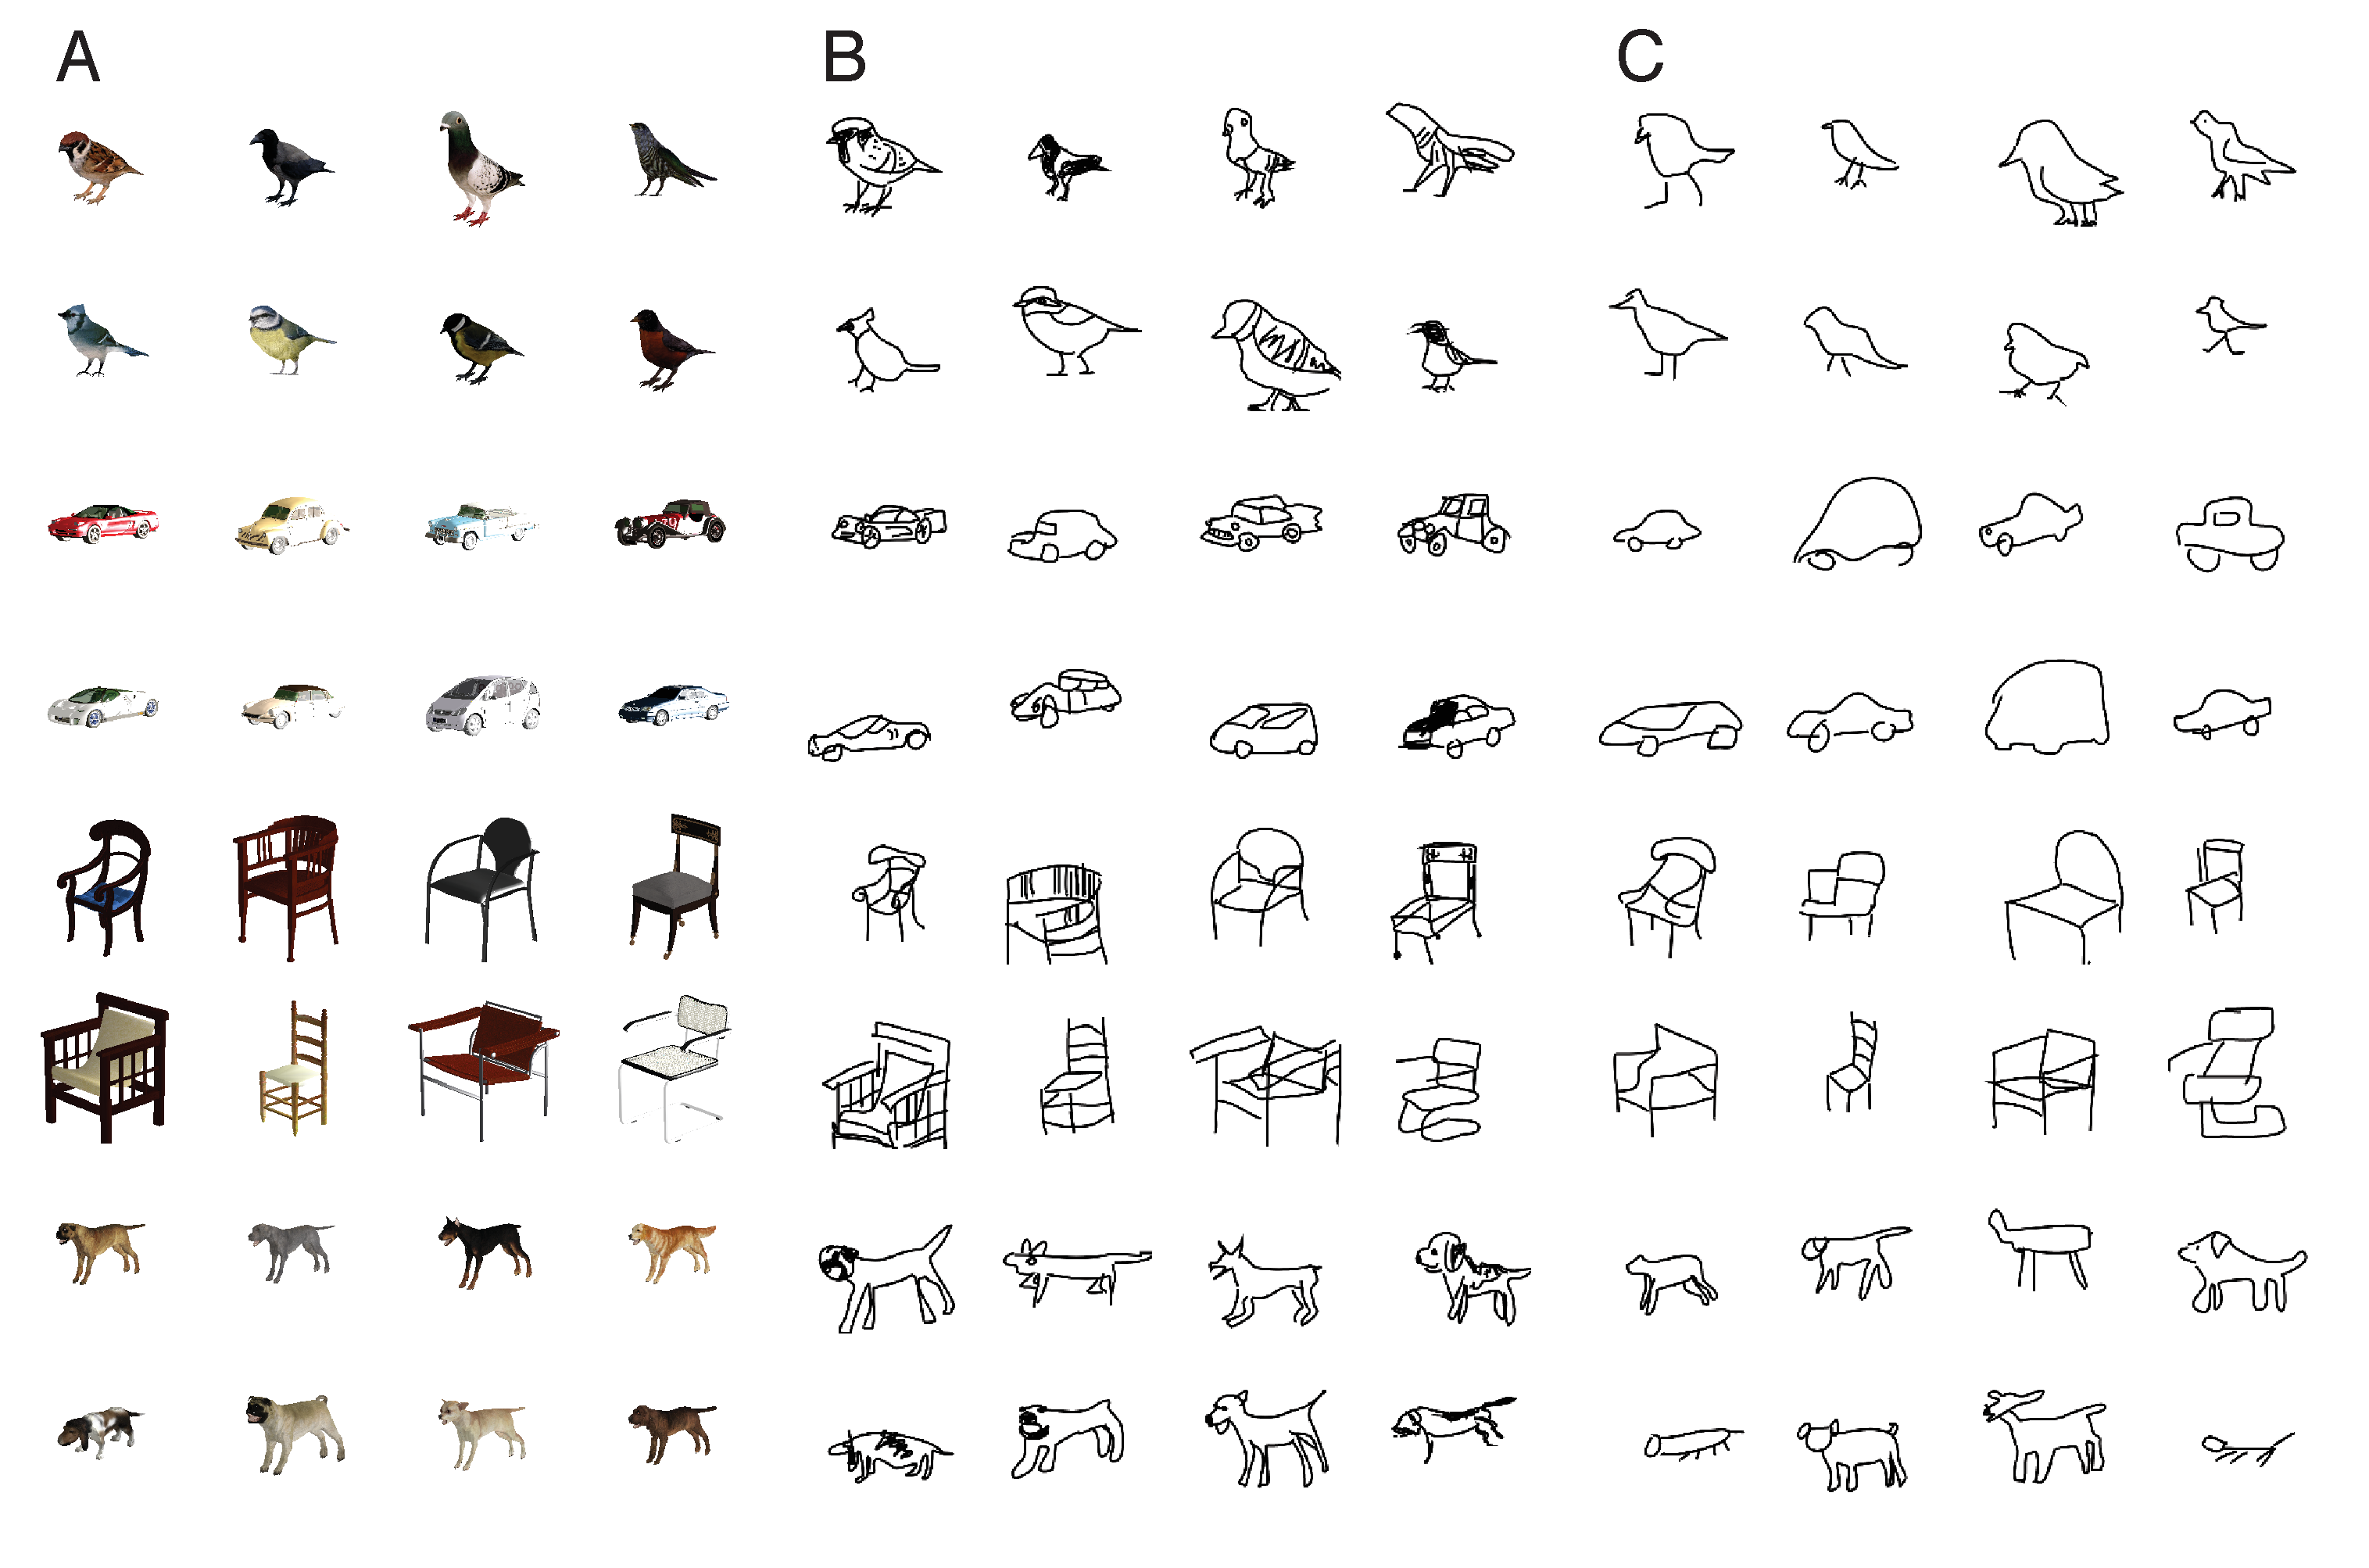
\includegraphics[width=0.95\textwidth]{figures/2_sketch_gallery.pdf}
\caption{(A) Object stimuli. (B) Example sketches produced in close condition. (C) Example skeches produced in far condition.}
\label{sketch_gallery}
\end{figure*}

Consistent with our prediction, we found that viewers were highly accurate overall at identifying the target from the sketches produced (proportion correct: 93.8\%, 95\% CI: [92.7\%, 94.8\%], estimated by bootstrap resampling participants). 
Moreover, we found that sketchers spent less time (close: 30.3s, far: 13.7s, \textit{p}$<$0.001), applied fewer strokes (close: 8.03 vs. far: 13.5, 95\% CI of difference: [3.75, 7.90], \textit{p}$<$0.001), and used less ink (proportion of canvas filled; close: 0.054, far: 0.042, 95\% CI: [0.01, 0.014], \textit{p}$<$0.001) to produce their sketches in the far condition than in the close condition. 
Despite the relative sparsity of sketches were in the far condition, viewers were near ceiling at identifying the target on these trials (far: 99.7\%, 95\% CI: [0.993, 0.999]; close: 87.9\%, 95\% CI: [0.858, 0.899]), and took less time to make these decisions than on close trials (far: 6.32 sec vs. close: 8.32 sec, 95\% CI: [-2.748, -1.251]).

\subsection*{Effect of context manipulation on sketch recognizability}

A natural explanation for the difference between close and far contexts in how costly the sketches were to produce is that they differed in how informative they were about identity of the target. Specifically, the greater time and ink spent on close sketches served to increase their degree of perceptual correspondence between the sketch and object, compared with less-costly far sketches, which exhibited a weaker correspondence to the target object in absolute terms, while still being communicatively effective in context. 
To investigate this possibility, another group of naive participants (N=112) was recruited to perform a sketch-object matching task, the data from which were used to estimate the strength of perceptual correspondence between each sketch and every object in the experiment. 
On each trial of this recognition experiment, participants were presented with a randomly sampled sketch and an image array containing all 32 objects, and were instructed to identify the object that best matched each sketch from the array. 
To obtain robust estimates of sketch-object perceptual correspondences, each sketch was presented approximately 10 times across different sessions. 
Consistent with possible explanation above, we found that close sketches were matched with their corresponding object rendering more consistently than far sketches were (close: 54.2\%; far: 37.5\%; $Z$=14.1, $p$<0.001), although both were successfully matched at rates greatly exceeding chance ($p$s < 0.001).

\begin{figure*}[htbp]
\centering
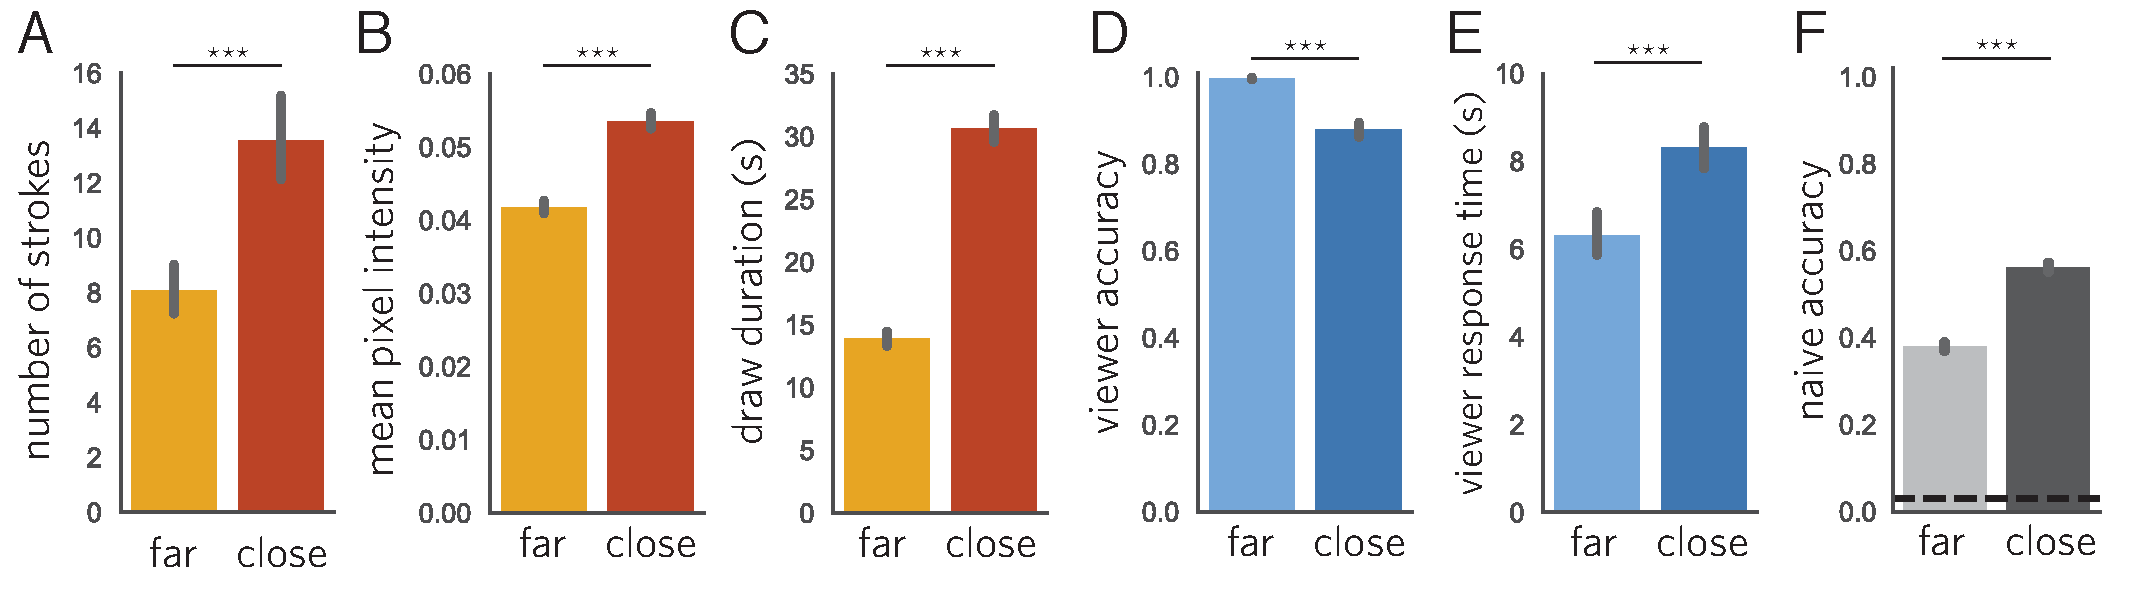
\includegraphics[width=0.95\textwidth]{figures/3_behavioral_performance.pdf}
\caption{(A-C) Sketchers used fewer strokes, less ink, and spent less time producing sketches in the far condition, relative to the close condition. (D-E) Viewers were at ceiling accuracy in identifying the target in the far condition, and were highly accurate in the close condition. (F) Naive matcher participants were more accurate for close sketches than far sketches.}
\label{task_performance}
\end{figure*}

%%% recognition experiments

%% Supplemental: report variation in different categories

%% Supplemental: report confusion matrix results: diagonal vs. off-diagonal block vs. rest of the matrix results.

% There was clear structure in the pattern of confusions for both close and far sketches. We further hypothesized that the particular way in which far sketches would differ perceptually from close sketches was that far sketches would be more confusable with other objects from the same basic-level category, while still being highly recognizable as a representation of the corresponding basic-level category.

% We measured this by comparing the within-category confusion rate to the overall confusion rate for close and far sketches, and found that XXX.

\subsection*{Computational model of sketch production in context}

The above findings suggest that human sketchers spontaneously account for information in common ground with their viewer, producing more informative sketches at the cost of additional time and ink in close contexts relative to far contexts. 
Observing such contextual flexibility argues against the notion that sketch production is constrained exclusively by the appearance of the target of depiction. 
Rather, these results suggest that information in common ground with the viewer plays a critical role in determining how informative and costly of a sketch people decide to produce during visual communication. 
And they suggest an analogy to how context influences how people produce linguistic utterances during verbal communication, a key target of contemporary theories of pragmatics in language use \cite{grice1975syntax,goodman2016pragmatic}.
Informed by these pragmatic theories, we propose that human sketchers determine what kind of sketch to produce in context by deploying two main faculties: \textit{visual abstraction}, which refers to the ability to judge how well a sketch evokes a real object, and \textit{pragmatic inference}, which refers to the ability to prefer sketches that are sufficiently detailed to be diagnostic of the target object in context, but no more detailed than necessary. 
Intuitively, this latter faculty can be decomposed into two aspects: context sensitivity, a preference for sketches that are diagnostic of the target relative to the distractors; and cost sensitivity, a preference for less costly sketches. 
To test this proposal, we developed a computational model of the sketcher that embodied both visual abstraction and pragmatic inference, and was instantiated as a probabilistic program ``wrapped'' around a deep convolutional neural network. 
Constructing such a model allowed us to evaluate the contribution of each component using formal model comparison, as well as quantitatively characterize the model's behavior in novel contexts.

\subsubsection*{Defining communicative utility of sketches}

We define a context, $O$, to be a set of objects containing a target, $t$, and three distractors, $D=\{d_1,d_2,d_3\}$:

\begin{equation} \label{object set}
O = \{t,D\}
\end{equation}

We define the sketcher $\mathcal{S}$, to be a decision-theoretic agent that prefers to produce a sketch of the target, $s_t$, proportional to its communicative utility, $U$, where the utilities of each sketch have been normalized over the space of producible sketches via the softmax function (Eq. \ref{sketcher_distribution}):

\begin{equation} \label{sketcher_distribution}
\mathcal{S}(s_t|t, D) \propto \frac {\exp [{U(s_t,t,D)]}} {\sum_{i=1}^{N} {\exp [U(s_i,t,D)]}}
\end{equation}

We introduce three variants of the sketcher, whose decision-making behavior is determined by their respective utility functions. 
In each variant, this utility consists of two terms which trade off against one another: an informativity term and a cost term. 

First, we define the utility function for a \textit{pragmatic} sketcher that is sensitive to both context and cost, $S_{2C}$, which estimates a sketch's informativity in terms of its \textit{diagnosticity} in context. 
A sketch's diagnosticity is defined by the natural log probability that an imagined viewer, $\mathcal{V}$, would select the target object given the sketch and all objects in context, $\ln \mathcal{V}(t|s,D)$. 
A sketch's cost, $C(s)$, is defined to be a monotonic function of the amount of time taken to produce it. 

\begin{equation} \label{sketcher_utility}
U_{S_{2C}}(s,t,D) = w_i \cdot \ln \mathcal{V}(t|s,D) - w_c \cdot  C(s)
\end{equation}
where $w_i$ and $w_c$ are independent scaling parameters that are applied to the diagnosticity and cost terms, respectively, and determine how strongly each term contributes to the overall utility of the sketch. 

The imagined viewer $\mathcal{V}$, in turn, is assumed to select the target object proportional to the perceptual correspondence between the sketch and the target, $\textrm{sim}(s,t)$, normalized by the correspondences between the sketch and all four objects in context, again via the softmax function:

\begin{equation} \label{literal_viewer_score}
\mathcal{V}(t|s,D) \propto \frac {\exp\{\alpha \cdot \textrm{sim(s, t)}\}} {\sum_{i=1}^{4} \exp\{\textrm{sim}(s,o_i)\}}
\end{equation}
where $\alpha$ is another scaling parameter determining the assumed optimality of the listener's decision policy: as $\alpha \rightarrow \infty$, the imagined listener is more likely to choose the object with highest perceptual correspondence to the sketch. Intuitively, this means that the viewer is more likely to pick the correct object when the sketch corresponds more strongly to the target than to the distractors. 

Second, we define the utility function for a \textit{context-insensitive} sketcher, $S_{sim}$, which replaces the diagnosticity term (defined in terms of the viewer) with a \text{resemblance} term reflecting the absolute degree of perceptual correspondence between a sketch and the target, $\textrm{sim}(s,o)$, and ignores the distractors. 

Third, we define the utility function for a \textit{cost-insensitive} sketcher, $S_{nocost}$, which sets the cost term to zero ($w_c=0$), and thus captures the aim to produce sketches that would be informative to an imagined viewer in context without regard for how much time they would take to produce. 

In our proposed sketcher model, $\mathcal{S}$, we define the informativity term to be a mixture of the purely diagnosticity-based definition employed by $S_{2C}$ and the purely resemblance-based definition employed by $S_{sim}$. 
To do this, we infer a mixture weight parameter, $w_{d}$, that interpolates between these two notions of informativity: 

\begin{equation} \label{prag_interpolation}
I(s,t,D) = w_{d} \cdot \ln \mathcal{V}(t|s,D) + (1-w_{d}) \cdot \textrm{sim}(s,t). 
\end{equation} 

Combining the utilities in this way captures the intuition that a communicative sketcher seeks to produce a sketch that both resembles the target object and distinguishes the target from the distractors.

After algebraically simplifying, the full utility is:

\begin{equation}
U(s,o) =  w_i \cdot  I(s,t,D) - w_c \cdot C(s)
\end{equation}

\begin{figure*}[htbp]
\centering
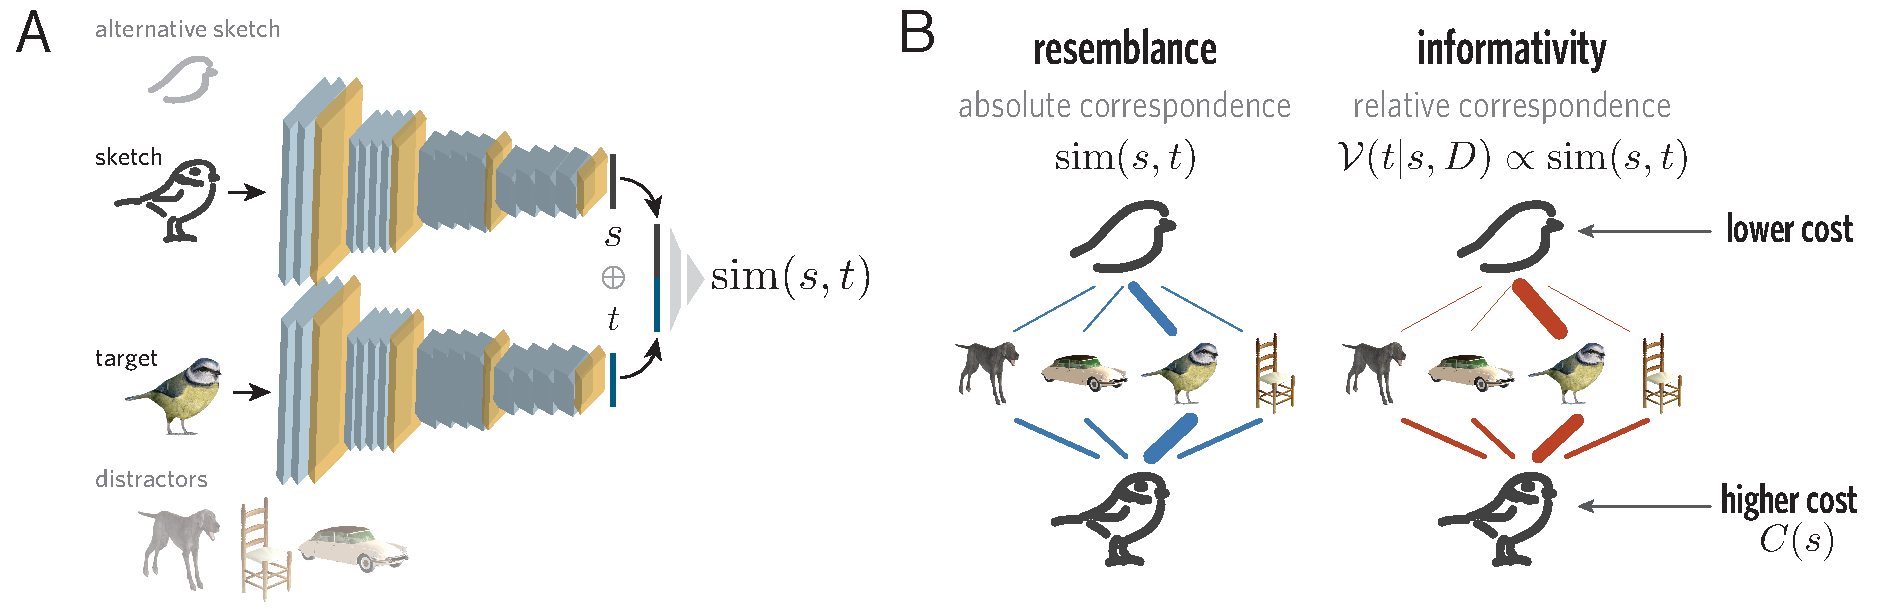
\includegraphics[width=0.95\textwidth]{figures/4_model_schematic.pdf}
\caption{(A) Architecture of visual encoder model for sketches and object renderings. Consists of pre-trained deep convolutional neural network (VGG-19) and shallow nonlinear ``adaptor'' neural network to evaluate sketch-object similarity. Takes sketch and object image as input, and outputs a similarity score reflecting how well the sketch resembles the object. Adaptor was trained on a subset of our dataset, and evaluated on held-out sketches. (B) Sketch-object correspondence computed for each object in context and each sketch in the test set. To determine the relative informativity of each sketch, the similarity scores between this sketch and all four objects were softmax normalized. The cost of each sketch was assumed to vary with the amount of time taken to produce it.}
\label{model_schematic}
\end{figure*}


\subsubsection*{Defining perceptual correspondence between sketches and objects}

In order for this sketcher to generate quantitative predictions, it needs to be able to compute the perceptual correspondence ($\textrm{sim}(s,o)$) for any sketch-object pair. 
We approached this problem in two ways: by employing human responses on the sketch-object matching task as an empirical approximation to $\textrm{sim}(s,o)$ for every sketch in our dataset, and employing a visual encoder model adapted to predict $\textrm{sim}(s,o)$, which was trained in a crossvalidated fashion on empirical estimates of $\textrm{sim}(s,o)$.

Informed by recent advances in computational vision \cite{FanCommon2018,yamins2014performance}, we instantiated the visual encoder as a deep convolutional neural network (DCNN). 
This choice of model class is motivated by prior work showing that such networks, in addition to being a type of universal function approximator \cite{hornik1991approximation}, learn higher-layer feature representations that capture high-level perceptual information in drawings \cite{FanCommon2018}, capture perceptual judgments of object shape similarity \cite{kubilius2016deep}, and predict neural population responses in categories across the ventral visual stream \cite{yamins2014performance} when trained on challenging natural object recognition tasks \cite{deng2009imagenet}. 
Consistent with this prior work, we hypothesized that higher layers of these networks would provide a superior visual feature basis for modeling human-like visual abstraction in this task, relative to the lower-level image statistics represented in earlier layers.

Concretely, the visual encoder is a function that accepts a pair of images as input: a sketch, $s$, and an object rendering, $o$, and returns a scalar value reflecting the degree of perceptual correspondence between the sketch and object, $\textrm{sim}(s,o)$, which lies in the range $[0,1]$, where $\textrm{sim}(s,o)=0$ reflects no correspondence and $\textrm{sim}(s,o)=1$ reflects maximal correspondence (Eq. \ref{visual_encoder}).

\begin{equation}
\label{visual_encoder}
\textrm{sim}(s,o) = a(b(s,o))
\end{equation}

This encoder consists of two functional components: a base visual encoder network, $b$, and an adaptor network, $a$. 
We employ VGG-19 pretrained to recognize objects from the Imagenet database as our base visual encoder, whose parameters remain frozen \cite{simonyan2014very}. 
We then augment the pretrained feature representation in a higher layer of VGG-19 (i.e., `fc6', the first fully-connected layer) with a shallow adaptor network, which is trained to predict the perceptual correspondence between specific sketch-object pairs. 
We train an adaptor network because while prior work has shown that the representation of object \textit{categories} converges for sketches and photos at higher layers in DCNN models trained only on photos \cite{FanCommon2018}, additional supervision can substantially improve the accuracy of predictions involving comparisons between sketches and photos at the \textit{image} level \cite{sangkloy2016sketchy}. 
We also train two additional adaptor networks appended to early and intermediate layers of VGG-19 (see Materials and Methods) in order to test the hypothesis, motivated by prior work, that higher-level visual features provide a better fit to human perceptual judgments than features from earlier layers \cite{kubilius2016deep}.
Critically, all adaptor networks contained approximately the same number of learnable parameters, and were trained on the same data using exactly the same optimization procedure for an equal number of epochs. 
All model evaluations involving the base encoder and trained adaptor network were performed in a fivefold crossvalidated manner, with the full communication task dataset split into training, validation, and test sets in a 80\%, 10\%, and 10\% ratio. 

Within this modeling framework, we conducted a series of targeted lesion studies to test each aspect of our hypothesis about the core cognitive faculties employed by humans to decide which sketch to produce in context. 
First, we evaluated the contribution of pragmatic inference by removing context sensitivity and cost sensitivity from the sketcher agent; these experiments relied upon empirical estimates of $\textrm{sim}(s,o)$. 
Second, we evaluated the contribution of visual abstraction by comparing how well higher-level vs. lower-level visual feature bases explained patterns of visual communication behavior.

\subsubsection*{Evaluating contribution of pragmatic inference}

% In each variant, this utility consist of two terms: an informativity term and a cost term. 
% First, we define the utility function for a context-sensitive and cost-sensitive sketcher, $S_{2C}$, which defines a sketch's informativity in terms of its diagnosticity in context. 
% A sketch's diagnosticity is defined by the natural log probability that an imagined viewer, $\mathcal{V}$, would select the target object given the sketch and all objects in context, $\ln \mathcal{V}(t|s,d)$. 
% A sketch's cost is defined to be a monotonic function of the amount of time taken to produce it $C(s)$. 

We hypothesized that a \textit{pragmatic} computational sketcher model that is sensitive to both context and cost would provide a strong fit to human sketch production behavior, as well as outperform lesioned alternatives lacking either component.
To test this hypothesis, we evaluated three model variants characterized by their distinct definitions of communicative utility: a pragmatic one sensitive to both context and cost ($S$), one \textit{not} sensitive to context but sensitive to cost ($S_{sim}$), and one that \textit{is} sensitive to context but \textit{not} sensitive to cost ($S_{nocost}$).
In this set of model evaluations, we employed empirical estimates of the correspondence between sketches and objects, $\textrm{sim}(s,o)$, to compute sketch diagnosticity in context. 
In this and subsequent model evaluations, we defined a sketch's cost, $C(s)$, to be a monotonic function of the amount of time taken to produce it.

Our goal was to ascertain how well each model could produce informative sketches and appropriately modulate its behavior according to the context condition, and not necessarily to reproduce exactly the same sketch as a particular participant had on a specific trial. 
As such, we aggregated all sketches of the same object produced in the same context condition when estimating their key functional properties (i.e., correspondence to objects and their cost to produce), so each sketch was represented by the mean in its object-context category. 
Model predictions were generated to the same level of granularity, in the form of a probability distribution over each of 64 categories of sketches, reflecting each combination of object and context condition (e.g., `basset sketch produced in a close context'). 

% latex table generated in R 3.5.1 by xtable 1.8-3 package
% Mon Oct 22 12:53:09 2018
\begin{table}[ht]
\centering
\begin{tabular}{lrrrrrr}
  \hline
split & \multicolumn{1}{p{0.35in}}{\centering cost (fc6)} & \multicolumn{1}{p{0.35in}}{\centering context (fc6)} & \multicolumn{1}{p{0.35in}}{\centering fc6 vs. conv42} & \multicolumn{1}{p{0.35in}}{\centering fc6 vs. pool1} & \multicolumn{1}{p{0.35in}}{\centering cost (human)} & \multicolumn{1}{p{0.35in}}{\centering context (human)} \\ 
  \hline
1 & 2.70 & 44.54 & 105.51 & 281.65 & 11.93 & 17.98 \\ 
  3 & 1.98 & 31.86 & 94.77 & 256.83 & 8.95 & 19.15 \\ 
  4 & -0.67 & 8.35 & 93.41 & 247.57 & 9.54 & 13.41 \\ 
  5 & 5.99 & 28.12 & 113.59 & 268.80 & 7.92 & 16.07 \\ 
  median & 2.34 & 29.99 & 100.14 & 262.81 & 9.25 & 17.02 \\ 
   \hline
\end{tabular}
\caption{Bayes Factors for different model comparisons across different splits}
\label{model_comparison}
\end{table}

To generate these predictions, first we employed Bayesian data analysis to infer a posterior distribution over the four latent scaling parameters in the model, applied to the informativity ($w_{i}$), cost ($w_{c}$), diagnosticity ($w_{d}$), and correspondence ($\alpha$) terms. 
Next, we presented each model with exactly the same set of contexts that were presented to human sketchers in the communication experiment, and evaluated the posterior predictive probabilities that each model assigned to sketches in every object-context category, marginalizing over the posterior distribution over latent parameters. 
We conduct these evaluations on each of the test sets from the same five crossvalidation folds that were used to train and test the visual encoder, to permit direct comparison of these two sets of modeling results. 

We found that the pragmatic sketcher, $S$, provided a much stronger overall fit to human behavior than the context-insensitive variant, $S_{sim}$ ($Bayes Factor (BF) = XX; w_d = YY$, 95\% credible interval $= [X, Y]$), and the cost-insensitive variant, $S_{nocost}$ ($BF = XX; w_c = YY$, 95\% credible interval $=[X, Y]$; see Table \ref{model_comparison}). 

To explore the behavioral patterns that may explain these differences in overall performance, we examined three aspects of each model's behavior: (a) \textit{sketch retrieval}: its ability to assign a high absolute rank to the target sketch category in context (out of 64 object-context alternatives);(b) \textit{context congruity}: its ability to consistently prefer the context-congruent version of the target object over the context-incongruent version (i.e., a close sketch of the target on a close trial); and (c) \textit{cost modulation}: how consistently it produced costlier sketches than average in the close condition, and less costly sketches than average in the far condition, mirroring human behavior

We found that in general, sketch classification performance was high for all three model variants (target rank 95\% CI: pragmatic = $[XX,XX]$, context-insensitive = $[XX,XX]$, cost-insensitive = $[XX,XX]$) (Fig.~\ref{model_results}A, left).

However, only the pragmatic sketcher was able to produce the sketch appropriate for the context condition (Fig.~\ref{model_results}B, left); neither the context-insensitive nor the cost-insensitive variants displayed this context congruity (95\% CI: pragmatic = $[XX,XX]$, context-insensitive = $[XX,XX]$, cost-insensitive = $[XX,XX]$). 
This was attributable to a bias shared by both the context-insensitive and cost-insensitive variant to produce sketches appropriate for a close context, because these sketches are highly informative, and thus higher in absolute utility if the distractors are ignored, or in the absence of a cost penalty. 

Moreover, only the pragmatic sketcher produced costlier sketches than average in the close condition (Fig.~\ref{model_results}C, left), and less costly sketches than average in the far condition (95\%CI: $[XX,XX]$). The context-insensitive variant is inherently unable to modulate the cost of the sketches it produces by context condition, and thus is no more or less likely to select a costlier, more diagnostic sketch on a close trial than a far trial (95\%CI: $[XX,XX]$). 
While the cost-insensitive variant did exhibit cost modulation by context, because it ignores their cost, preferred costlier sketches overall in both contexts (95\%CI: $[XX,XX]$). 

Together, these results suggest that both context and cost sensitivity are critical for capturing key aspects of contextual flexibility in human visual communication. 

\begin{figure*}[htbp]
\centering
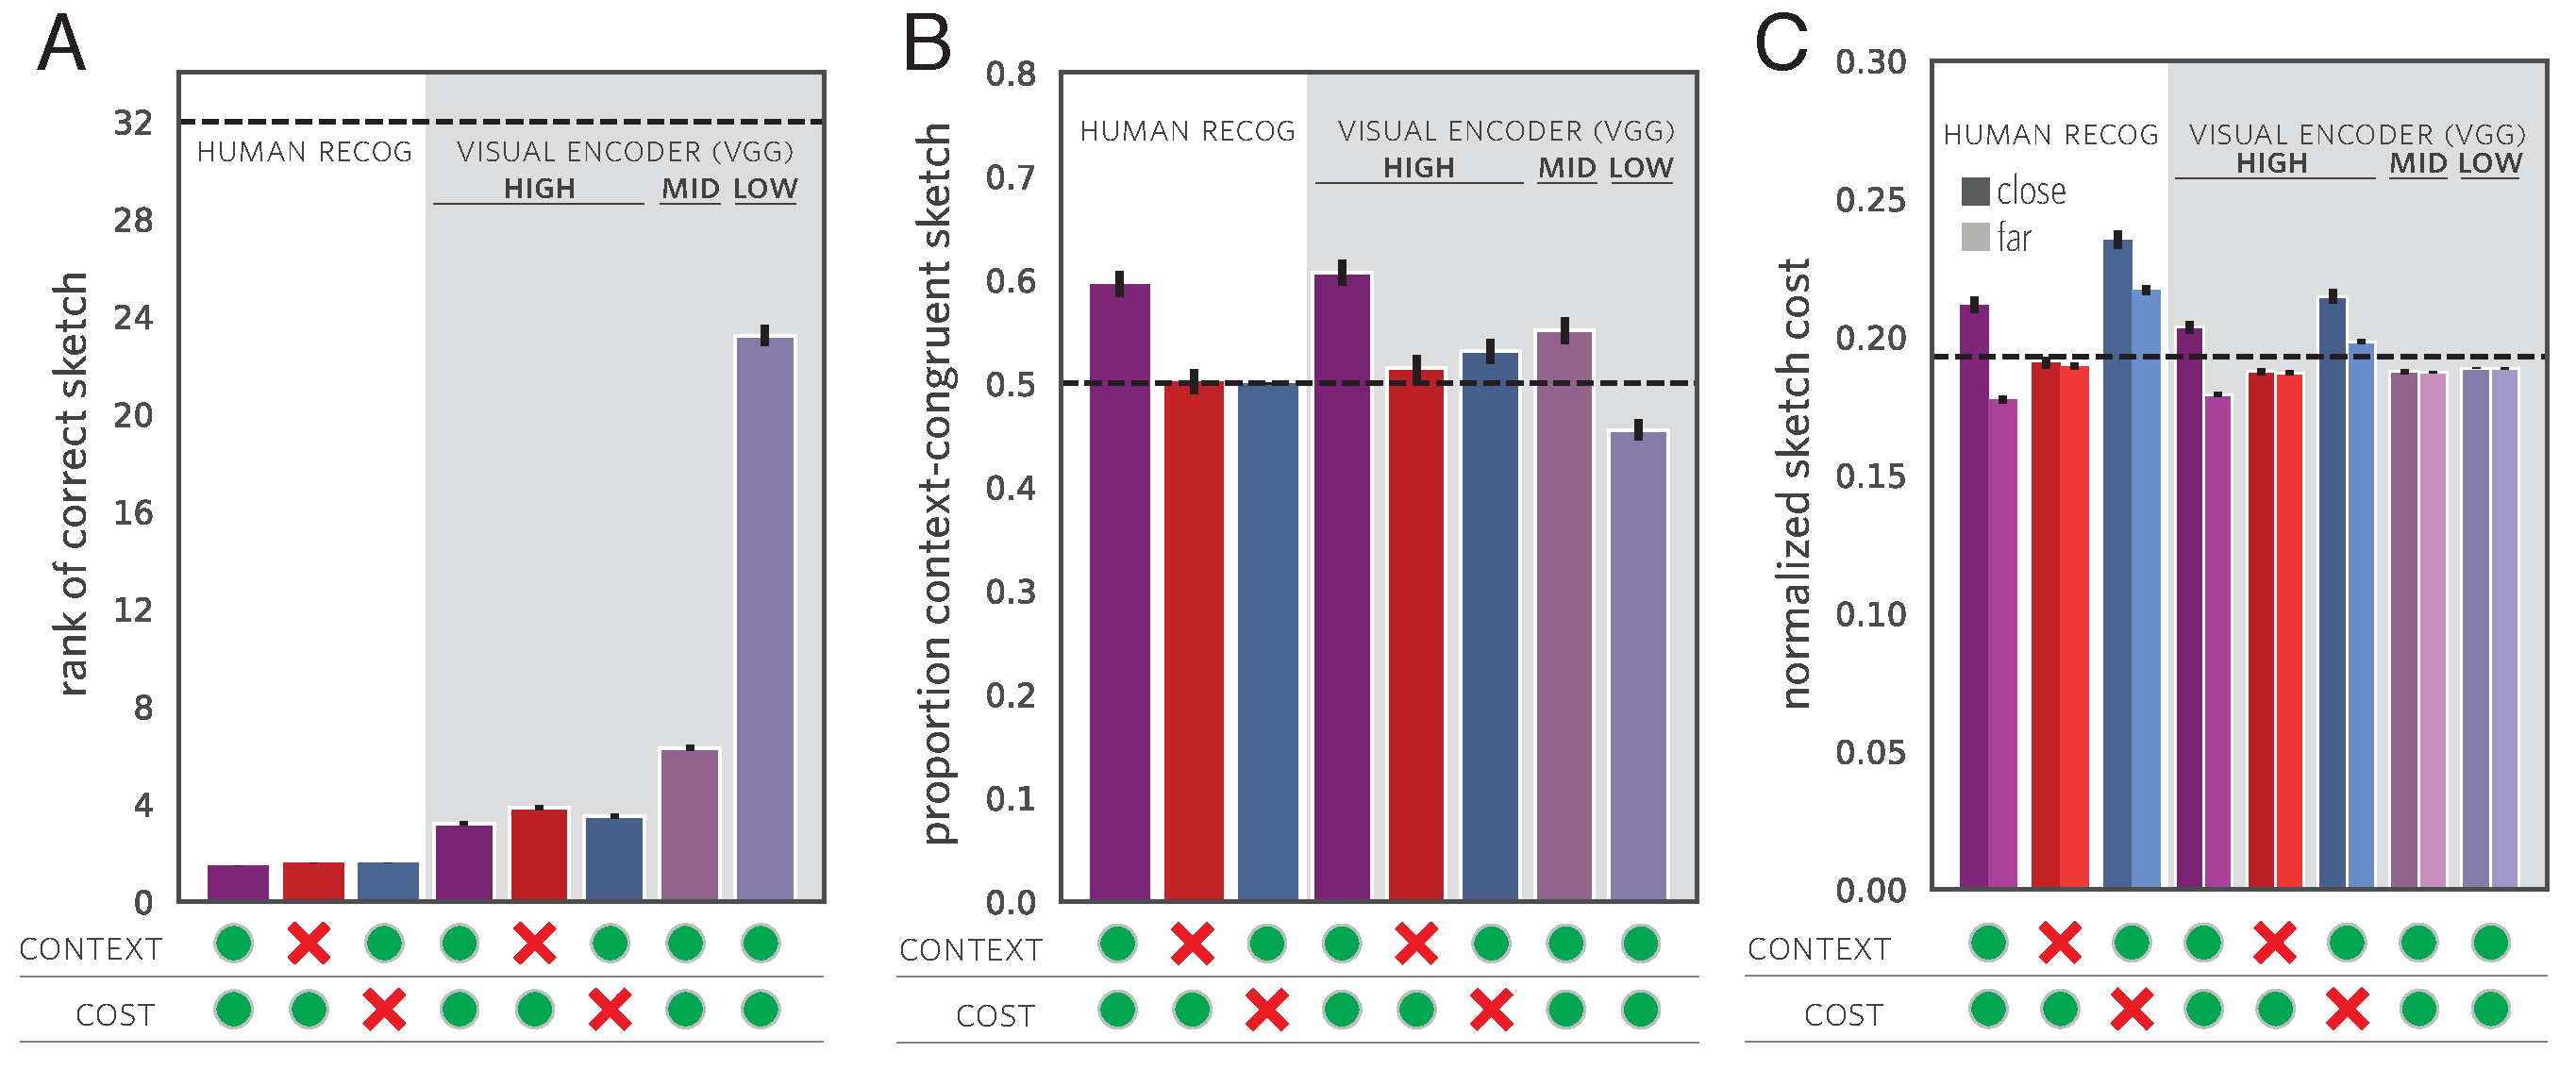
\includegraphics[width=0.99\textwidth]{figures/5_model_results_2.pdf}
\caption{Sketch production behavior by model variant. The table below each panel indicates whether the corresponding model variant plotted above is sensitive to context or cost. A green disc indicates context/cost sensitivity; a red `X' indicates the lack of context/cost sensitivity. 
Results in lefthand region of each panel (white background) reflect model predictions when using empirical estimates of $sim(s,o)$ based on human sketch recognition behavior. 
Results in the righthand region (gray background) reflect model predictions when using variants of the DCNN visual encoder, the adaptor components of which were trained in a five-fold crossvalidated manner using human sketch recognition behavior. 
All results reflect average model behavior on test data only across identical train-test splits. 
Error bars represent 1 s.e. for this average estimate, found by applying inverse-variance weighting on individual confidence intervals from each train-test split. 
A: Rank of target sketch in list of 64 object-context categories, ordered by the probability assigned by each model. 
Dashed line reflects expected target rank under uniform guessing. 
Distribution of target rank scores across models suggest that high-quality estimates of $sim(s,o)$ are critical for strong performance. 
B: Proportion of trials on which each model assigned a higher rank to the context-congruent sketch of the correct object than the context-incongruent version of the correct object. 
Dashed line reflects indifference between the two versions of the sketch. 
Only models above this line show consistent and appropriate modulation of sketch producton by context. C: Relative time cost of sketches produced by each model, after applying min-max normalization to raw draw duration measurements. 
Predicted sketch cost on each trial computed by marginalizing over probabilities assigned to each sketch category. 
Darker bars reflect behavior in the close condition; lighter bars the far condition. 
Dashed line indicates the average cost of sketches in the full dataset; bars below this line reflect a preference for sketches that are less costly than average, bars above this line for sketches that are costlier than average. 
Only models that span this dashed line match the pattern of contextual modulation of sketch cost displayed by human sketchers.}
\label{model_results}
\end{figure*}

\subsubsection*{Evaluating contribution of visual abstraction}

Having established the importance of pragmatic inference for explaining contextual flexibility during visual communication, we next sought to evaluate the contribution of visual abstraction. 
To accomplish this, we incorporated a visual encoder into our computational model of the sketcher, instantiated as a deep convolutional neural network (i.e., VGG). 
Having an encoding model that operates directly on image inputs is important for a computational theory of visual communication because it allows our full model to generate predictions in novel contexts, without the need to collect new empirical estimates of sketch-object correspondence. 
In particular, we hypothesized that generalization to novel communication contexts would be supported by a visual encoder that uses high-level features to predict sketch-object correspondences, rather than lower-level features from earlier or intermediate layers of the neural network. 
To test this hypothesis, we compared three variants of the best-performing pragmatic sketcher model above that used visual features adapted from different layers of the neural network: \textit{high-level}, \textit{mid-level}, and \textit{low-level}.
We followed the same procedure as above to generate model predictions for the test set of each crossvalidation fold of our dataset, such that disjoint sets of sketches and communicative contexts were used to train each visual encoder and evaluate them. 
 
Consistent with our hypothesis, we found that a pragmatic sketcher model employing high-level features provided a better fit to the data than one using mid-level features (high vs. mid BF: $[X.XX, X.XX]$), which in turn outperformed a model using low-level features from an early layer (mid vs. low BF: $[X.XX, X.XX]$). 
These results suggest that making fuller use of the depth of VGG to compute the perceptual correspondence between a sketch and object yields a stronger basis for predicting and explaining human visual communication behavior.

Critically, using high-level features supported strong performance on sketch retrieval (target rank: $[X.XX, X.XX]$, Fig.~\ref{model_results}A), compared to mid-level features (target rank: $[X.XX, X.XX]$) and low-level features (target rank: $[X.XX, X.XX]$). 
These results show that without a high-performing visual encoder, the model is much less likely to produce sketches of the correct object, a basic prerequisite for successful visual communication even in the absence of contextual variability. 

Moreover, the pragmatic sketcher model using high-level features also displayed context congruity (95\% CI: $[XX,XX]$, Fig.~\ref{model_results}B), comparable in degree to the best-performing pragmatic model that lacked an encoder, showing that our full sketcher model was able to successfully reproduce this key signature of contextual flexibility for novel communicative contexts and sketches. 
The variant using mid-level features also displayed context congruity to a weaker extent (95\% CI: $[XX,XX]$), suggesting that an intermediate level of visual abstraction could achieve an intermediate degree of context congruity. 
By contrast, the variant using low-level features failed to prefer the context-congruent sketch category (95\% CI: $[XX,XX]$), providing a lower bound on the level of visual abstraction required in the underlying vision model to support visual communication behavior. 

Again, only the pragmatic sketcher model using high-level features displayed the same pattern of cost modulation as the best-performing pragmatic model lacking an encoder (95\%CI: close = $[XX,XX]$, far = $[XX,XX]$, Fig.~\ref{model_results}C), while both of the other variants using mid-level and low-level features failed to do so (95\%CI: mid-level: close = $[XX,XX]$, far = $[XX,XX]$; low-level: close = $[XX,XX]$, far = $[XX,XX]$).  

Having identified the best-performing visual encoder as the one that adapted features from a higher layer of VGG, we then performed the same context and cost sensitivity lesion experiments as before in order to evaluate the contribution of pragmatic inference in our full model. 
We found that removing context and cost sensitivity led to only modest decrements in overall sketch retrieval performance (95\% CI: $[XX, XX$, Fig.~\ref{model_results}A), suggesting that the visual encoder itself is a major determinant of the ability to produce sketches of the correct object, whether or not the context-congruent version). 
However, removing context and cost sensitivity greatly diminished the ability of this model to produce the context-congruent sketch of the correct object (context-insensitive 95\% CI: $[XX,XX]$; context-insensitive 95\% CI: $[XX,XX]$, Fig.~\ref{model_results}B), and approriately modulate the cost of the sketches it produced (context-insensitive 95\% CI: $[XX,XX]$; context-insensitive 95\% CI: $[XX,XX]$, Fig.~\ref{model_results}C). 
Taken together, these results converge with those of the lesion experiments conducted on the pragmatic sketcher model without a visual encoder, and provide strong evidence for the importance of both visual abstraction and pragmatic inference for explaining contextual flexibility in human visual communication. 

\section*{Discussion}

In this study, we explored how communicative context influences real-time natural visual communication behavior. We found that ... We collected a rich behavioral dataset and developed an integrated computational model that explains contextual flexibility in human visual communication by combining constraints from perception and pragmatic reasoning.

% literatures that this should connect to: other graphical communication papers


% limitations of this work


% future directions

Together, this work provides the first unified computational theory of how perception and social cognition support contextual flexibility in real-time visual communication.

\subsubsection*{Code availability} The code for the analyses presented in this article is publicly available in a Github repository at: \url{https://github.com/judithfan/visual_communication_in_context}.

\subsubsection*{Data availability} The data presented in this article are publicly available in a figshare repository.

\subsection*{Supporting Information (SI)}

% The main text of the paper must stand on its own without the SI. Refer to SI in the manuscript at an appropriate point in the text. Number supporting figures and tables starting with S1, S2, etc. Authors are limited to no more than 10 SI files, not including movie files. Authors who place detailed materials and methods in SI must provide sufficient detail in the main text methods to enable a reader to follow the logic of the procedures and results and also must reference the online methods. If a paper is fundamentally a study of a new method or technique, then the methods must be described completely in the main text. Because PNAS edits SI and composes it into a single PDF, authors must provide the following file formats only.

\matmethods{

\subsection*{Communication experiment: Manipulation of context in sketch-based reference game}

\subsubsection*{Participants}

A total of 192 unique participants, who were recruited via Amazon Mechanical Turk (AMT) and grouped into pairs, completed the experiment. They were provided a base compensation of \$X.XX for participation and earned a \$X.XX bonus for each correct trial. In this and subsequent behavioral experiments, participants provided informed consent in accordance with the Stanford IRB.

\subsubsection*{Stimuli}

Stimuli were thirty two 3D mesh models of objects belonging to 4 categories (i.e., birds, chairs, cars, dogs), containing eight objects each. Each object was rendered in color on a gray background at three-quarter perspective, 10$^{\circ}$ viewing angle (i.e., slightly above), and fixed distance.

\subsubsection*{Task}

Drawings were collected in the context of an online, sketching-based reference game (``Guess My Sketch!''). The game involved two players: a \textit{sketcher} who aims to help a \textit{viewer} pick out a target object from a set of distractor objects by representing it in a sketch. On each trial, both participants were shown an array of the same four objects; however, the positions of these objects were randomized for each participant. On each trial, one of the four objects was highlighted on the sketcher's screen to designate it as the target.\mwu{maybe add some text on why it is important to randomize.}

Sketchers drew using black ink on digital canvas (pen width = 5 pixels; 300 x 300 pixels) embedded in a web browser window using Paper.js (http://paperjs.org/). Participants drew using the mouse cursor, and were not able to delete previous strokes. Each stroke of which was rendered on the viewer's screen immediately upon the completion of each stroke. There were no restrictions on how long participants could take to make their drawings. After clicking a submit button, the viewer guessed the identity of the drawn object by clicking one of the four objects in the array. Otherwise, the viewer had no other means of communicating with the sketcher. Both participants received immediate task-related feedback: the sketcher learned which object the viewer had clicked, and the viewer learned the identity of the target. Both participants earned bonus points for each correct response.

For each pair, objects were grouped into eight quartets: Four of these quartets contained objects from the same category (``close''); the other four of these quartets contained objects from different categories (``far'' condition). \mwu{show picture of each condition?} Each quartet was presented four times, such that each object in the quartet served as the target exactly once. The assignment of objects to quartet and condition was randomized across pairs.

Successful communication was primarily quantified as the viewer's accuracy in identifying the target. The investment of time was measured as the length of time between the beginning of the first stroke to the completion of the final stroke in each sketch, and the investment of ink was measured in two ways: as the number of strokes used for each sketch and the proportion of the drawing canvas filled by ink.

\subsection*{Recognition experiment: Measuring perceptual similarity between sketches and objects}

\subsubsection*{Participants}

A total of 112 participants were recruited via Amazon Mechanical Turk (AMT). They were provided a base compensation of \$1.00 for their participation, and earned an additional \$0.01 bonus for each correct response.

\subsubsection*{Task}

On each trial, participants were presented with a randomly selected sketch collected in the sketch-based reference game, surrounded by a grid containing the 32 objects from that experiment. Their goal was to select the object in the grid that best matched the sketch. Participants were instructed to prioritize accuracy over speed. A small proportion of outlier trials that were either too fast (response latency <1000ms) or too slow (>30s) were filtered from the dataset; we reasoned that behavior on such trials was likely to be noisier and not comparable to that on the remainder of trials.\mwu{is this kosher?} The removal of these outlier trials did not have a substantial impact on the pattern of recognition behavior. In order to mitigate the possibility that participants could adjust their matching strategy according to any particular sketcher's style, each session was populated with 64 sketches sampled randomly from different reference games. Participants were provided with binary feedback about the correctness of their response on each trial via a bonus counter that incremented by 1 point for each correct identification, but did not change for incorrect trials.

% VERIFY THIS: Participants were permitted to complete multiple sessions of this task, but were prevented from providing identification judgments for the same sketch twice, or for sketches they themselves had produced or viewed (on the rare occasion that this participant had also participated in the reference game experiment).

\subsection*{Computational modeling}

We hypothesized that two core cognitive competencies are necessary and sufficient for explaining contextual flexibility in this visual communication task: (1) visual abstraction, the capacity to perceive the high-level perceptual correspondence between an object and a drawing of it; and (2) social inference, the ability to infer what information would help a viewer distinguish the target from distractors.

Our goals in developing a computational model of sketch production in this visual communication task were to: (a) to formalize this hypothesis in a manner that can generate quantitative predictions even in novel contexts; and (b) evaluate the contribution of the hypothesized components to explaining the observed pattern of human behavior.\mwu{i think this is interesting -- why make a computational model? expand more maybe? are we claiming that this is how humans think?}

Towards the first goal, we propose a framework for instantiating visual abstraction and social inference by combining a deep convolutional neural network visual encoder with a probabilistic model of recursive social inference. Towards the second goal, we formally compare how well the full model predicts human behavior to a targeted set of lesioned variants, and examine how each component influences the observed pattern of behavior.  

\subsubsection*{Visual encoder module}

% \mwu{this section is a huge brain dump - need more sentences to tie paragraphs together.}

The visual encoder module accepts a pair of images, a sketch and an object rendering (both 224 by 224 RGB images), as input and returns a scalar value in the range $[0,1]$, reflecting the degree of perceptual correspondence between the sketch and object. This module consists of two components: a base visual encoder and an adaptor network.

We employ VGG-19 \cite{simonyan2014very} as our base visual encoder, a high-performing and widely used deep convolutional neural network architecture. This network had been pretrained to categorize objects on the ImageNet database, which contains millions of photographs from hundreds of object categories \cite{deng2009imagenet}. Despite the fact that drawings are highly abstracted away from natural visual inputs, prior work has shown a striking isomorphism in the similarity structure \cite{kriegeskorte2008matching} of object categories in sketches and photos at higher layers in these models \cite{FanCommon2018}, without any additional training. While these deep nets excel at (and were indeed optimized for) categorization of objects, two additional competencies are required to succeed at the visual communication task described above. First, an observer must be able to represent fine-grained differences between different images of objects from the same category; second, this observer must also be able to discern image-level correspondences between sketches and photos of the same object.\mwu{maybe we can say: image-level differences are easy -- we can use VGG off the shelf. To dscern fine-grain detail, we need an adaptor.}

In order to better approximate the granularity with which human observers can distinguish different images, we augment VGG-19 with a shallow fully-connected \textit{adaptor} network that is trained to adapt the generic visual feature representation computed by VGG-19 to predict the perceptual correspondence between individual sketches and objects. Here only the parameters of this adaptor network are trained and we do not finetune the base visual encoder. This approach has been successfully used in prior work to better predict human semantic categorization judgments \cite[]{peterson2016adapting}, and to improve sketch-based photo retrieval \cite[]{sangkloy2016sketchy}.

To explore the degree to which the \textit{visual abstraction} afforded by the complex transformations applied by successive layers of VGG-19 are required to capture human behavior during visual communication, we train three adaptor networks that intercept VGG-19 image representations at different layers: the first max pooling layer (early), the tenth convolutional layer (mid), and the first fully connected layer (high). \mwu{add something about early being edges, high being object recognition masks, etc.} To facilitate comparison between adaptor networks, we ensured that each of the three contain a comparable number of trainable parameters (Table~\ref{table:parameters}) with identical training hyperparameters (learing rate, batch size, etc.). To discriminate which layer provides the best starting feature basis for predicting sketch-object correspondence, these adaptor networks were also deliberately constrained to be shallow, i.e., consisting only of two linear layers with an intervening point-wise nonlinearity.

In the following, we provide a detailed description of the architecture and hyperparameter choices for each adaptor. We refer to the respective adaptor network as: \textit{early-adaptor}, \textit{mid-adaptor}, and \textit{high-adaptor}.

\begin{table}
\centering
\begin{tabular}{| l | c |}
\hline
Model & Parameters \\
\hline
\hline
early-adaptor & 1048839 \\
\hline
mid-adaptor & 1049115 \\
\hline
high-adaptor & 1048833 \\
\hline
\end{tabular}
\caption{Number of parameters in the visual encoder modules.}
\label{table:parameters}
\end{table}

Two 4096-dimensional feature vectors are extracted for the sketch and object from the first fully-connected layer ($fc6$) of VGG-19. These two vectors are then concatenated to form a single 8192-dimensional vector, to be passed into the high-adaptor network. The high-adaptor architecture is composed of a linear layer from 8192 to 128, followed by a ``swish'' nonlinearity \footnote{Swish is a recent nonlinearity found via reinforcement learning-based search shown to work better than ReLU for deep models on a suite of tasks.} \cite[]{ramachandran2018searching} and dropout, then another linear layer from 128 to 1.

In practice, we find the ability of the model to fit the data is robust to the choice of nonlinearity (alternative nonlinearities were TanH and ReLU) and size of hidden layer, within the range $(2^{7},2^{9})$).

Similarly, the mid-adaptor consists of a linear layer of 1024 to 1021, swish, dropout, then a linear layer from 1021 to 1. Although 1021 seems like a peculiar choice, we want to ensure that the number of trainable parameters in mid-adaptor is as close to that of high-adaptor as possible. In this case, 1021 hidden units in the first layer is the most suitable choice. Since features from the 10th convolutionary layer of VGG are three dimensional (512 by 28 by 28), we first ``flatten" the input into a one dimensional vector of size 512 using a weighted linear combination $\sum_{i=1}^{28}\sum_{j=1}^{28} w_{ij} * x_{ij}$, where $x_{ij}$ represents a cross-section from VGG. The parameters  $\{w_{ij}|1\leq i,j \leq 28\}$ are learned jointly with the parameters of mid-adaptor. Intuitively, this is akin to attention over the spatial features of the 10th convolutional layer of VGG. We separately attend over 3D-object and sketch spatial features, creating two vectors of size 512, then concatenate prior to mid-adaptor.

Finally, the early-adaptor is almost identical to the mid-adaptor, except each feature is of size 64 by 112 by 112. Explicitly, this network starts with a linear layer of 4096 to 7875 (like the mid-adaptor, 7875 is chosen to match the number of parameters), swish, dropout, then a linear layer form 7875 to 1. Due to the input size, each attention module in early-adaptor has 12,544 learnable weights.

\paragraph{Sketch data preprocessing.} We filter the sketch dataset used to train each adaptor network to include only sketches that were correctly identified during the communication task (6.2\% incorrect) and were compliant with task instructions by not including `drawn' text annotations (4.4\% non-compliant). This filtered sketch dataset was then split into training, validation, and test sets in a 80\%, 10\%, and 10\% ratio, and this split was performed in a 5-fold cross-validated manner. Splits were based on context, defined as the set containing a specific target object and three distractor objects, such that no context appeared both in the training and test splits of any cross-validation fold. Specifically, we ensured that: (1) the number of sketches from each category (i.e. car) and \todo{clarification: equating number of `car' instances or number of `bluesport' instances within `car' category?} (2) the number of sketches from close and far trials were equated across splits. This was done to mitigate biases in accuracy due to imbalances in the training or test set.

% In the visual communication dataset, there is a close context and a far context. The former includes 4 objects of the same category (i.e. 3 distractor cars and 1 target car) whereas the latter includes 4 objects of different categories (i.e. a target car and a dog, chair, and bird as distractors).

\begin{figure}[h!]
\centering
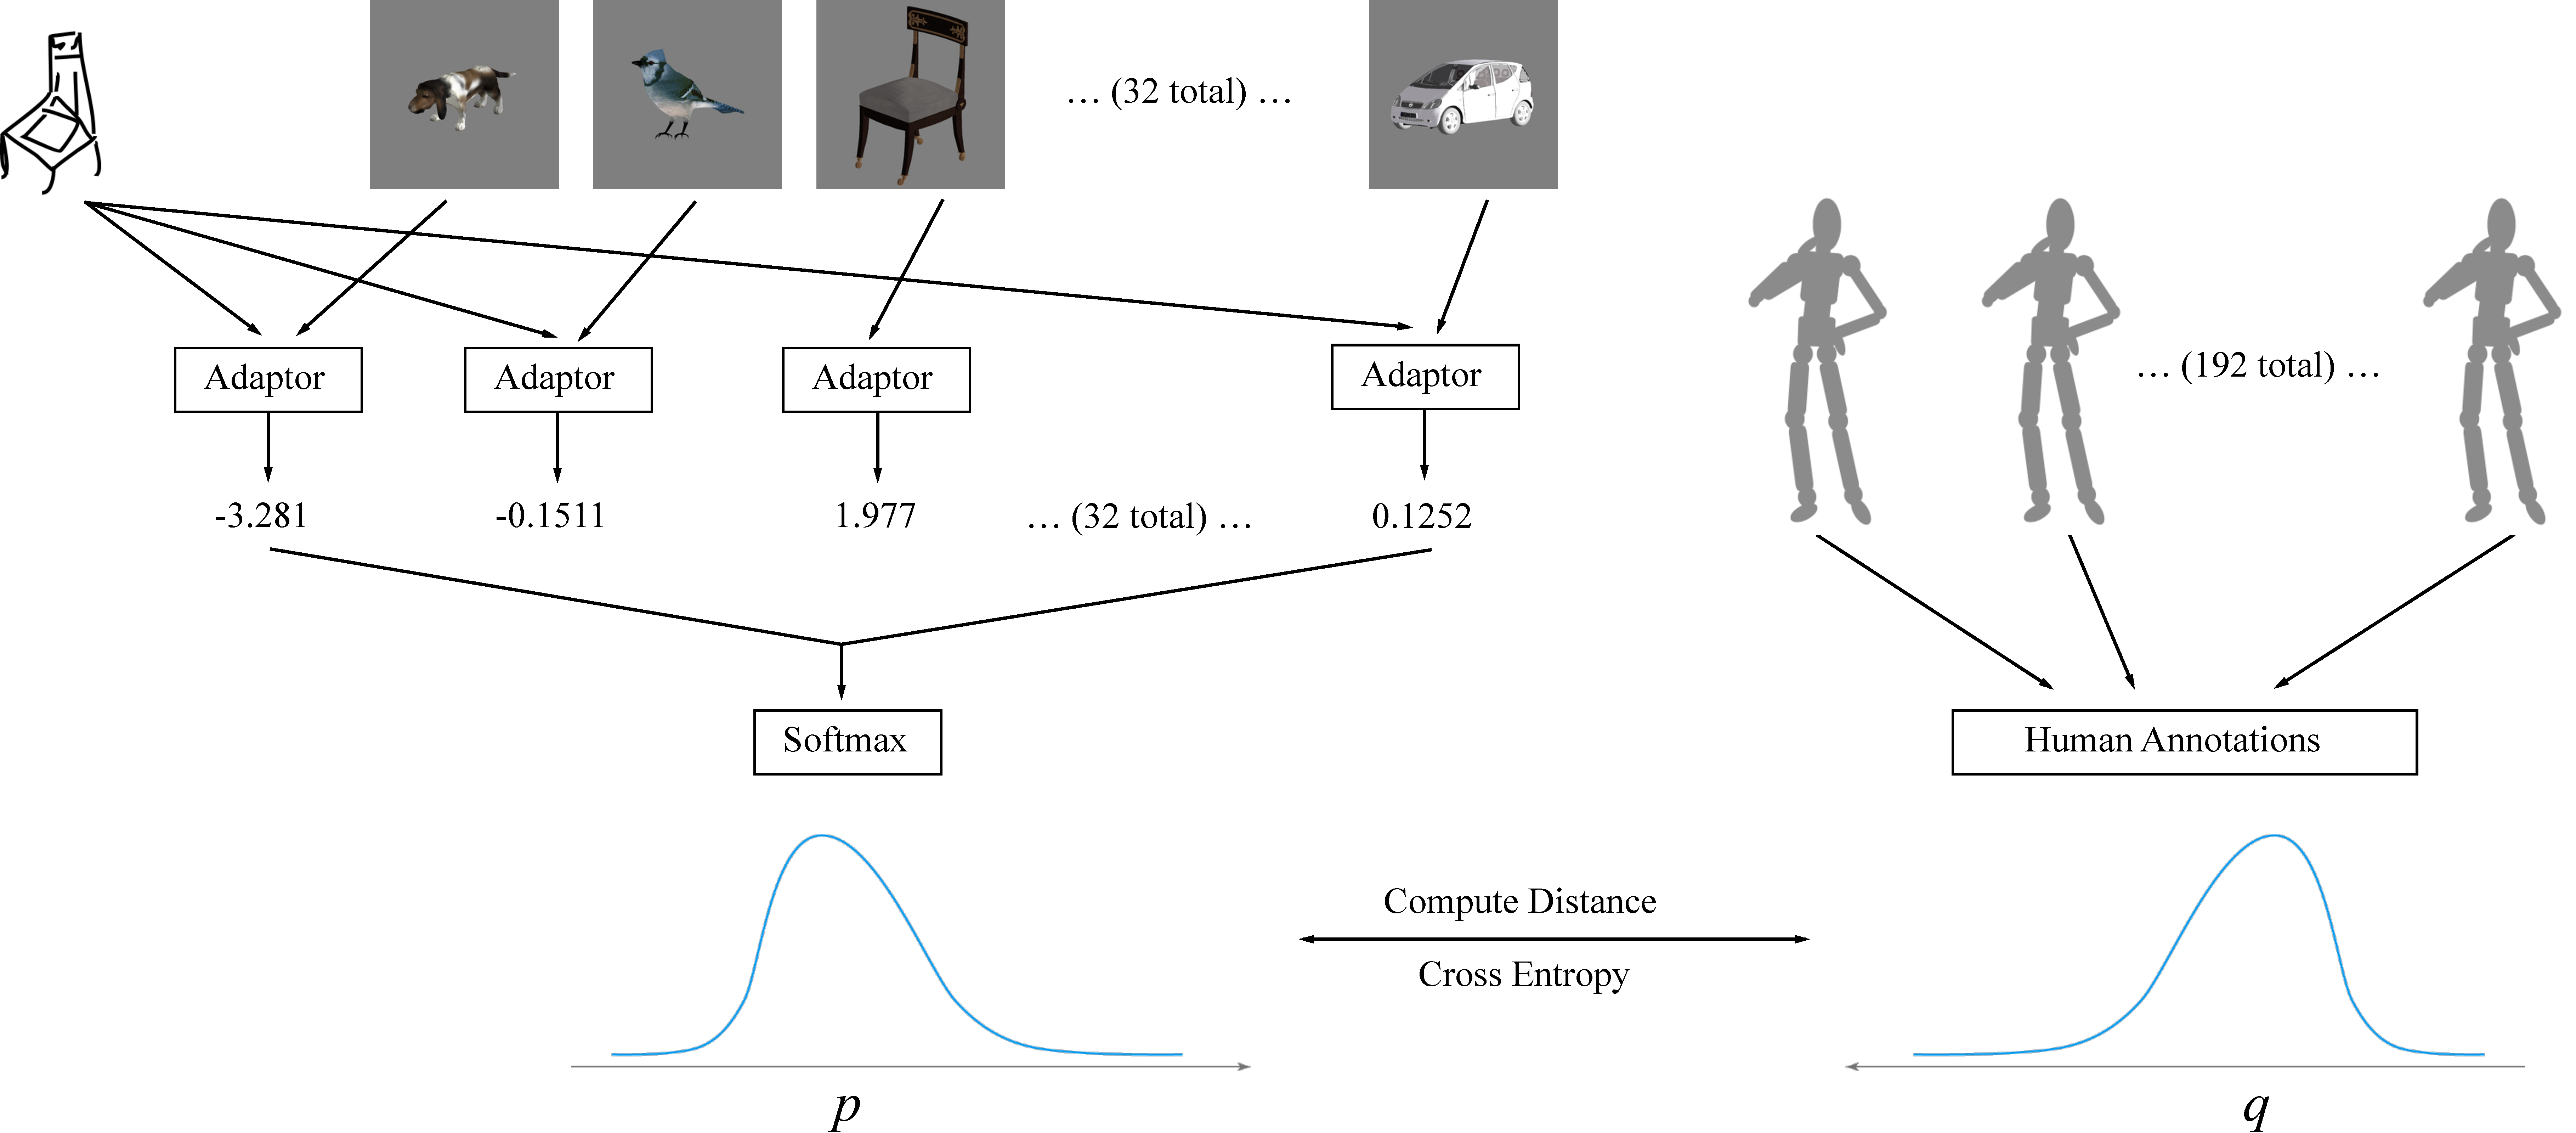
\includegraphics[width=0.95\columnwidth]{figures/adaptor_algorithm.pdf}
\caption{The adaptor measures similarity between a given sketch and 3D object rendering. To train the adaptor, we can minimize the distance between the distribution induced from a softmax over similarities and the human annotations.}
\label{fig:adaptor_training}
\end{figure}

\paragraph{Adaptor network training procedure.}
We now describe the training procedure for each visual encoder. Each adaptor network accepts a sketch-object pair as input and returns a real number as output, reflecting their perceptual correspondence. We construct a similarity vector of size 32 between a sketch and each object in the domain $\mathcal{I}$ (32 total), and apply a softmax on top to induce a probability distribution over objects. We define a loss function, $\mathcal{L}$, as the cross entropy between the induced distribution, $q$ and a empirical distribution of human recognition responses, $p$:

\begin{equation}
    \mathcal{L} = \sum_{x \in \mathcal{I}} p(x)\log q(x)
    \label{eqn:cross_entropy}
\end{equation}

The empirical response distribution was derived by computing the proportion of trials from the recognition experiment on which all sketches from the same context-object category (e.g., all sparrow sketches produced on close trials) was matched with each object. As a consequence, this response distribution not only provides an estimate of the strength of the match between a sketch and its corresponding object, but also the pattern of confusions that human observers exhibit, thus creating a more detailed profile of recognition behavior for each adaptor to match.

We use the Adam optimization algorithm \cite[]{kingma2014adam} with a learning rate of 1e-4 and minibatch size of 10 for 100 epochs, where an epoch is a full pass through the training set. As a property of the input domain, the gradients with respect to adaptor parameters are very small (1.51e-4 $\pm$ 2.61e-4), inevitably resulting in poor learning (we can reproduce this effect from several intializations). We find that naively increasing the learning rate led to unstable optimization, but that multiplying the loss by a large constant $C$ leads to a much smoother learning trajectories and good test generalization\footnote{Increasing the learning rate and multiplying the loss by a constant are not equivalent for second moment gradient methods.}. In practice, $C =$ 1e4. After training each adaptor for 100 epochs, we freeze the model with the best performance on a validation set. For each 3D object and sketch pair in the test set, we evaluate the perceptual correspondence and provide this as input to the social inference module, described next.

\mwu{We split the datasets of images and sketches into three groups: a training set, a validation set, and a test set. Post training, we use the parameters from the epoch with the highest validation accuracy i.e. early stopping ADD CITATION. During training, the model never sees any test data.}

\subsubsection*{Social inference module}

The social inference module must be able to evaluate the degree of perceptual correspondence between each object in context and any sketch it could produce, where the set of producible sketches consists of those in the test set (i.e., not used to train the visual encoder). Using this information, it outputs a distribution of scores over all test-set sketches, where the scores reflect each sketch's relative communicative utility.

Combining the two modules, we can define the sketcher, $\mathcal{S}$ to be a decision-theoretic agent that produces sketches, $s$, by soft-maximizing a utility function, $U$, given a particular object referent, $o$:

\begin{equation}
\mathcal{S}(s|o) \propto \exp\{{U(s,o)\}}
\end{equation}

The utility function of our context-sensitive sketcher, $U_{S_1}$, trades off the extent to which a given sketch is informative to an imagined viewer, $\mathcal{V}$, with the cost of producing that sketch, $C(s)$. This notion of informativity is defined by the (natural log) probability that a viewer would select the true object given the sketch and all objects in context. In our experiments, the cost of a sketch is operationalized as the amount of time taken to produce it, though in principle other metrics could be used (e.g., the number of strokes, proportion of canvas filled).

\begin{equation} 
U_{S_1}(s, o) = w_i \ln \mathcal{V}(o|s) - w_c C(s)
\end{equation}
where $w_i$ and $w_c$ are latent parameters weighting the influences of the sketch's perceptual properties and cost, respectively.

The viewer ($\mathcal{V}$) is assumed to decide between objects in context proportional to the perceptual correspondence between each object and the current sketch, $\textrm{sim}(s,o)$, which is scaled by a latent parameter $\alpha$.

\begin{equation} 
\mathcal{V}(o|s) \propto \exp\{\alpha \cdot \textrm{sim(s, o)}\}
\end{equation}
where $\alpha$ is a scaling parameter determining the assumed optimality of the listener's decision policy: as $\alpha \rightarrow \infty$, the listener is more likely to choose the object with highest perceptual correspondence to the sketch.

We also consider a \textit{context-insensitive} sketcher $S_0$ agent that aims to maximize the absolute perceptual correspondence between their sketch and the target, without taking the  distractors into account. Accordingly, the utility function of this context-insensitive sketcher is defined in terms of $\textrm{sim}(s,o)$ instead of informativity to $\mathcal{V}(o|s)$.

In our full sketcher model we combine these two agents by inferring a mixture weight parameter, $w_{prag}$, that interpolates between their two utilities:  

\begin{equation} 
I(s,o) = w_{prag} \cdot \ln \mathcal{V}(o | s) + (1-w_{prag}) \cdot \textrm{sim}(s,o)
\end{equation}

Combining the utilities in this way captures the intuition that a communicative sketcher seeks to produce a sketch that both resembles the target object and distinguishes the target from the distractors.

After algebraically simplifying, the full utility is:

\begin{equation}
U(s,o) =  w_p \cdot  f(s,o) - w_c \cdot C(s)
\end{equation}

\subsubsection*{Generating model predictions}

Each communication task trial is defined by a context containing four objects and a sketch. There are two attributes of each trial that are required for any variant of our model to be able to generate predictions given a context: (1) the perceptual correspondence between the sketch to each object in context and (2) the cost of producing the sketch.

We evaluate our model using both empirical and model-based approaches to measuring perceptual correspondence. For each sketch and context in a test set, the empirical perceptual correspondence between the sketch and a given object in context is defined as the proportion of recognition task trials on which all sketches from the same object-context category were matched to this object out of context. As such, all correspondence scores lie in the range $[0,1]$ and sum to 1 for sketches in the same object-context category:

$$\sum_{n=1}^{32} \textrm{corr} (s,o_{n}) = 1 $$,

where $n$ represents the $nth$ object in the stimulus set. $s$ refers to sketches from the same object-context category (i.e., depict object $o$ in context $c$, which can be either close or far). Because recognition responses are aggregated across all sketches within the same object-context category to compute the proportions above, this yields 32 sketch categories x 32 objects x 2 contexts = 2048 empirical perceptual correspondence scores in total.

Model-based perceptual correspondence scores are defined to the same level of granularity, with all sketches from the same object-context category sharing the same perceptual correspondence to a particular object, under a particular choice of visual encoder module (i.e., vgg-high, vgg-mid, vgg-low).

To compute this score for a particular visual encoder module and object, each test-set sketch from a given object-context category is passed in with this object to the visual encoder module, yielding a single image-level correspondence score lying in the range $[0,1]$. These image-level correspondence scores are then averaged across all sketches belonging to the same object-context category, yielding 32 objects x 32 sketches x 2 contexts  = 2048 model-based perceptual correspondence scores for each visual encoder module.

We measured the cost of each sketch empirically as the amount of time taken by the participant to produce it during the communication task. We reasoned that drawing time would be both a natural and straightforward way of measuring the cost of sketching for workers on Amazon Mechanical Turk, who increase their total compensation by completing tasks in a timely manner. However, as there were no absolute constraints on the amount of time that could be spent on each trial, there was considerable variability across different participants in terms of how much time they spent producing their sketches. To control for this variability across participants and to ensure robust estimates, we first removed outliers (draw times exceeding 5 s.d. from the mean), then z-score normalized drawing times across all remaining trials within a participant, and finally averaged these normalized draw times across sketches within the same object-context category as above, yielding 32 objects x 2 contexts = 64 empirical cost estimates in total.

\subsubsection*{Model comparison}

In order to test the contribution of each component of our sketcher model, we conducted a series of lesions as formal model comparisons.
To quantify the evidence for one model over another, we computed Bayes Factors:
the ratio of likelihoods for each model, integrating over all their respective parameters under the prior:
$$BF = \frac{\int P(D | M_1, \theta_1)P(\theta_1)}{\int P(D | M_2, \theta_2)P(\theta_2)}$$
Unlike classical likelihood ratio tests, which use the maximum likelihood, the Bayes Factor naturally penalizes models for their complexity \cite{rouder}.
We placed uninformative uniform priors over all five parameters required to specify our models: a discrete choice of the vision model used to compute perceptual correspondance
$$m \sim \textrm{Unif}\{\textrm{``pool1''}, \textrm{``conv42''}, \textrm{``fc6''}, \textrm{``empirical''}\}$$
and continuous parameters
$$w_p, w_c, w_{prag}, \alpha \sim \textrm{Unif}(0, 50)$$
as described in the previous section. To compute the likelihood function $P(D | M, \theta)$ for a speaker model $M$ under parameters $\theta$, we perform exact inference for our sketcher model using (nested) enumeration and sum over our data set (a test split of held-out sketches).

There are several possible methods to approximate Bayes Factors when exact evaluation of the integral is intractable. We compare two independent methods to check robustness of our estimate: annealed importance sampling and exact enumeration over a discretized grid of parameters. Annealed importance sampling (AIS; \cite{neal2001}) is a Monte Carlo algorithm that is commonly used to estimate the partition function, or marginalized likelihood, of probabilistic models. Because the integral is dominated by a typical set near the region of high likelihood, AIS uses an MCMC chain to construct a sequence of intermediate distributions interpolating between a tractable initial distribution (in our case, the prior) and intractable target distribution: we set the number of steps to 2000 and take the expectation over 48 independent samples from this procedure for every model of interest, using the implementation provided in the probabilistic programming language WebPPL. We can then obtain Bayes Factors to compare models by taking ratios of these estimates.

We compare our results from AIS to a more exact but brute-force approach: computing the exact likelihood at every point on a discrete grid of parameters.
This is of particular interest for nested model comparisons, e.g. comparing our full model to a no-cost variant.
Rather than computing the full marginalized likelihood for both models, we can use the Savage-Dickey method \cite{WagenmakersEtAl10} to simply compare the posterior probability against the prior at the nested point of interest (e.g. $w_c = 0$) for the full model.

We begin by comparing the full model using empirically estimated perceptual correspondences against nested ``no-cost'' ($w_c = 0$) and ``no-context'' ($w_prag = 0$) lesions. We then proceed to compare the three vision models derived from different layers of neural networks, marginalizing over all other parameters. Finally, we perform the same comparisons against cost and context lesions for the best-performing setting of the vision model (using ``fc6'').

\subsubsection*{Evaluating model predictions}

To further interpret the findings of our model comparison, we examined posteriors over the inferred parameters of the best-performing model and also computed posterior predictives to evaluate its behavior on several measures of interest:
\begin{enumerate}
    \item absolute rank of target class
    \item probability assigned to sketches from the congruent context, i.e. $$P(\textrm{`close' sketches} | \textrm{`close' context)} + \textrm{P(`far' sketches} | \textrm{`far' context})$$
    \item mean cost of predicted sketches
\end{enumerate}
We use MCMC to draw 1000 samples from the joint posterior with a lag of YYY, discarding XXX burn-in samples.
We constructed posterior predictive distributions by computing the measure of interest on the data set at every sample.
To estimate standard errors to statistically compare predictions across models, we employed a multi-stage bootstrapping procedure controlling for three nested sources of variability: estimation of measures on the data for a particular parameter setting and test split, variation across the parameter posterior for a test split, and variation across test splits.
We implemented our models and conducted inference in the probabilistic programming language WebPPL (Goodman \& Stuhlmuller, 2014).
All code necessary to reproduce our model results are available at the project github.

}

\showmatmethods % Display the Materials and Methods section

\acknow{Thanks to Dan Yamins and the Stanford CoCo Lab for helpful comments and discussion.}

\showacknow{} % Display the acknowledgments section

% \pnasbreak splits and balances the columns before the references.
% Uncomment \pnasbreak to view the references in the PNAS-style
% If you see unexpected formatting errors, try commenting out \pnasbreak
% as it can run into problems with floats and footnotes on the final page.
%\pnasbreak

% Bibliography
\bibliography{references}

\end{document}
